%%%%%%%%%%%%%%%%%%%%%%%%%%%%%%%%%%%%%%%%%%%%%%%%%%%%%%%%%%%%%%%%%%%%%%
% nuthesis-template.tex - Miguel A, Lerma - 3/31/2013
%                         mlerma@math.northwestern.edu
%%%%%%%%%%%%%%%%%%%%%%%%%%%%%%%%%%%%%%%%%%%%%%%%%%%%%%%%%%%%%%%%%%%%%%

%%%%%%%%%%%%%%%%%%%%%%%% DISCLAIMER %%%%%%%%%%%%%%%%%%%%%%%%%%%%%%%%%%
% 
% In spite of the effort to accommodate this template and the nuthesis
% class to the official requirements of the university to write a 
% Ph.D. dissertation, it is not possible to guarantee that it will 
% always work, and the author of the dissertation remains responsible
% for checking that such requirements are actually fulfilled by 
% his/her final work.
%
%%%%%%%%%%%%%%%%%%%%%%%%%%%%%%%%%%%%%%%%%%%%%%%%%%%%%%%%%%%%%%%%%%%%%%


\documentclass[12pt]{nuthesis}	% The nuthesis class is based on 
				% amsbook.cls.
				
\usepackage[english]{babel}
\usepackage[utf8x]{inputenc}
\usepackage[T1]{fontenc}
\usepackage[natbibapa]{apacite}
\usepackage{comment}
\usepackage{todonotes}
\usepackage{graphicx}
\usepackage[toc]{appendix}
\usepackage{amsmath}




%%%%%%%%%%%%%%%%%%%%%%%%%%%%%%%%%%%
% DATA OF AUTHOR AND DISSERTATION %
%%%%%%%%%%%%%%%%%%%%%%%%%%%%%%%%%%%

\author{Matthew Heston}

\title{The Effect of Availability, Message Attributes, and Relational Variables on Predicting Mobile Responsiveness}

%\degree{DOCTOR OF PHILOSOPHY}  % Default: DOCTOR OF PHILOSOPHY

\field{Technology and Social Behavior}            % Default: Mathematics

%\graduationmonth{June}         % The default is June or December
                                % depending on current date.

%\graduationyear{2003}          % Default: current year.


				% Use \includeonly to select the 
%\includeonly{chap1,chap2,...}	% chapters to include if you are 
				% using the \include command below.
				% This way you can latex only a the 
				% part you are working on, which 
				% is faster than latexing the entire 
				% thesis. 


\begin{document}
%	
%	THE BODY OF YOUR THESIS STARTS HERE
%

%%%%%%%%%%%%%%%%%%%%%%
% Some initial stuff %
%%%%%%%%%%%%%%%%%%%%%%

\frontmatter		% Preliminary pages start here.

\maketitle		% Produces the title page.

\copyrightpage		% Creates the copyright page.


\abstract		% Abstract.

Responsiveness -- the time it takes for a message recipient to respond to a message -- has long been of interest to scholars in the fields of computer-mediated communication and human-computer interaction. It has been hypothesized that responsiveness is used to signal emotional information, and many empirical studies have demonstrated that violating expectations about responsiveness is associated with negative evaluations. The increasing use of mobile devices for messaging complicates our understanding of how people decide when to respond to a message. While early work focused on desktop computers and the workplace, the rise of mobile messaging means people can be reached anywhere, at any time, and likely from many different types of contacts they communicate with on their device. As a result, the decision of responding immediately or delaying response is affected by many previously unconsidered factors.

To understand how much these different factors affect mobile responsiveness, 92 Android phone owners from around the United States were recruited to participate in this project. Both log data and questionnaire data were collected using a custom built Android app that participants ran on their phones for 7 days. 1,635 session initiation SMS messages were analyzed using a series of multilevel regression models. Results indicate that a user's subjective rating of their availability at the time a message was received is strongly associated with responsiveness. Message attributes, such as how important a message is to the person who received it, have modest effects on responsiveness. Certain types of messages were also associated with much longer delays in responsiveness. Relational variables, such as how close the message recipient is to the message sender, were not found to have large effects on responsiveness. 

\acknowledgements	% Acknowledgements (optional).

Text for acknowledgments.



%% A few more optional pages (uncomment if needed)
%
\listofabbreviations
\noindent
CMC --- Computer Mediated Communication \\
ESM --- Experience Sampling Method \\
FtF --- Face-to-face conversation \\
SIP --- Social Information Processing Theory \\
SIA --- Session Initiation Attempt
%
%This is the list of abbreviations (optional).
%
%\glossary
%
%This is the glossary (optional).
%
%\nomenclature
%
%This is the nomenclature (optional).
%
%% Note that the dedication text must be passed as an argument
%% of the \dedication command
%\dedication{This is the dedication (optional).}
%

\clearpage\phantomsection % needed for the hyperlinks to work correctly
\tableofcontents	% Table of Contents will be automatically
			% generated and placed here.

\clearpage\phantomsection % needed for the hyperlinks to work correctly
\listoftables		% List of Tables and List of Figures will be placed

\clearpage\phantomsection % needed for the hyperlinks to work correctly
\listoffigures		% here, if applicable (optional).



\mainmatter             % Actual text starts here.

%%%%%%%%%%%%%%%%%%%%%%%%%%%
% Actual text starts here %
%%%%%%%%%%%%%%%%%%%%%%%%%%%

% If there is an introduction it must be the first chapter

\chapter{Introduction}

Everyday conversation is an important part of how relationships develop and are maintained~\citep{baxter1987symbols,duck1999relating}. Communicators enter these everyday interactions with expectations about how to interact~\citep{burgoon1993interpersonal} which in turn guides both their behavior and their understanding of one another~\citep{burgoon1993effects}.

The near ubiquity of mobile devices is likely affecting how these interactions occur. Over 90\% of U.S. adults own a cell phone of some kind, with nearly 70\% owning a smart phone~\citep{anderson2015technology}. Although owners of these devices use them for many different purposes, mobile messaging remains the most widely used application~\citep{duggan2015mobile,smith2015us}. People use these apps frequently throughout the day~\citep{battestini2010large} to communicate with a variety of different types of contacts, from family to friends to acquaintances to work colleagues~\citep{church2013s,min2013mining} for a variety of different purposes, including just killing time~\citep{pielot2015boredom}, coordinating plans~\citep{ling200210}, and relational maintenance~\citep{cui2016beyond,pettegrew2015smart}.

One way mobile devices affect interpersonal communication and expectations in these interactions are that they result in a mismatch of information relevant to conversation initiation between the initiator and the recipient, i.e., the initiator doesn't know whether or not the recipient is available to talk. This is not entirely unique to mobile devices. A landline caller, for example, does not know whether or not the call recipient is home or not before he attempts to call. However, mobile devices are unique in that they relax certain assumptions about the recipient's state. The landline caller would not bother calling if they assumed the receiver was not home. A worker might not send a work email to a colleague after 5:00pm, or at least not expect a response that night if they did, since they might assume the colleague does not check work email after work. Mobile devices are distinct from these other media in that their owners carry devices with them nearly constantly~\citep{oksman2003perhaps,rainie2015americans,turkle2008always}, and, as a result, may be thought of as constantly reachable. \citet{wellman2001computer} refers to this as a shift in communication from ``place-to-place'' to ``person-to-person.''

The combination of this mismatch in information and assumptions of constant availability is problematic for users of mobile messaging systems such as SMS because it results in differences in the meaning of responsiveness -- the time it takes for a message recipient to respond to a message -- to senders and receivers. Message senders often expect a quick reply~\citep{laursen2005please}, interpret delays in responsiveness as meaningful~\citep{rettie2009mobile}, and feel ignored when their responsiveness expectations aren't met~\citep{church2013s}. Message receivers, on the other hand, reportedly are trying to control how much time they spend on their phone~\citep{ames2013managing,smith2015us}, and may prioritize certain messages as needing an immediate response while delaying response to certain messages or contacts~\citep{cui2016beyond,wohn2015ambient}.

To better understand these differences between senders' and receivers' attitudes towards mobile responsiveness, we need a better model of how much different factors affect a message recipient's response time. There are many plausible factors which affect responsiveness decisions. Given that they can be reached at any time, a device owner may simply be in a situation where they cannot reasonably respond~\citep{avrahami2007improving}. Even if they are available, mobile messaging users have expressed various types of information they consider when deciding whether or not to respond immediately, such as how important the message is to them~\citep{cui2016beyond} and their relationship with the person contacting them~\citep{wohn2015ambient}. However, no quantitative studies to date have measured the effects of these different variables on responsiveness. Prior quantitative work on response time has focused on workplace platforms such as email~\citep{dabbish2005understanding} and instant messaging~\citep{avrahami2006responsiveness,avrahami2008waiting}, and as a result has not studied responsiveness in the ``always on'' context of mobile messaging.

Knowing how much different factors affect responsiveness allows us to form better theoretical models describing differences between message sender expectations and message receiver action. If, on average, the primary reason mobile messaging users do not respond to a message has little to do with message prioritization but instead with simply not being available to respond, responsiveness may be understood in terms of what \citet{krauss1996social} call an ``encoder/decoder model'' of communication, and responsiveness could be considered a type of noisy signal. In other words, the reason users report being upset about being ``ignored''~\citep{church2013s} could be because they cannot properly decode the meaning of responsiveness. If, on the other hand, message receivers' responsiveness decisions are driven largely by their interpretation of the received message, or by their relationship with the person contacting them, then responsiveness might be better understood by what \citet{krauss1996social} call a ``dialogic model'' of conversation, where responders adjust behavior to convey different meaning based on their conversational context.

These perspectives in turn have practical implications for the design of communication platforms. If it were the case that a lack of immediate response is most often the result of unavailability, the ``noisy signal'' of responsiveness may be strengthened by providing more information to a message sender. If the sender could see, for example, that their intended recipient is currently at a movie theater, they are more likely to interpret lack of fast responsiveness as indicating unavailability since the recipient is in a location where they cannot access their device. If, on the other hand, responsiveness is driven largely by sender--receiver relationship, maintaining plausible deniability may be more important to message recipients, so they can later make excuses to certain contacts about why they were unable to respond~\citep[as in][]{aoki2005making, hancock2009butler}.

The goal of this dissertation is to measure the effects of availability, message attributes, and relational variables on mobile responsiveness. Using SMS data and experience sampling data collected using a custom developed Android application from smart phone owners around the United States, the current work aims to contribute to our understanding of how these different factors affect responsiveness behavior in mobile messaging.

\chapter{Background}

\section{Nonverbal Cues in Computer-Mediated Communication}
\label{sec:cues}

A useful way to think about responsiveness is as a nonverbal cue in CMC. In face-to-face (FtF) communication, humans use a variety of nonverbal cues such as appearance, touch, gaze, and proximity~\citep{burgoon2016nonverbal} which have been shown to be important in many areas, such as social influence~\citep{hogg2006social}, conflict resolution~\citep{ting2001managing}, and interpersonal attraction~\citep{burgoon1991relational,erceau2007tactile}. While CMC communicators sometimes have to rely more on verbal cues~\citep{walther2005let}, nonverbal cues still serve an important role in engaging in CMC interactions~\citep{lo2008nonverbal,tidwell2002computer,walther1992interpersonal}. Empirical work has shown that responsiveness conveys some of the same types of information as other nonverbal behavior, such as personality and trust~\citep{kalman2013online}, and viewing responsiveness as a nonverbal behavior allows us to draw on the long history of nonverbal behavior research in considering the role of responsiveness in CMC.

The seeming lack of nonverbal cues (such as gaze and touch) was central to early theoretical approaches to CMC. Social Presence Theory~\citep{short1976social} described all media as fitting on a one-dimensional spectrum of \textit{social presence}, which refers to ``the degree of salience of the other person in an interaction''. Greater social presence was often tied directly to the nonverbal cues present in FtF interaction~\citep[e.g.,][]{burgoon1984relational}, such that CMC, and especially text-based interaction, were thought to result in less social presence. It was also hypothesized that communicators would choose an appropriate medium for their message, e.g., avoid communicating potentially ambiguous message over a less rich medium given the higher likelihood of being misinterpreted~\citep{daft1986organizational}.

Such theories comprise what \citet{walther2002cues} refer to as ``cues filtered out'' theories of CMC, so called because of their emphasis on the lack of nonverbal cues driving behavior. Instead, Social Information Processing theory (SIP)~\citep{walther1992interpersonal}, rejects the notion that the lack of certain nonverbal cues restricts communicators' abilities. 

Conceptual models of social cognition in psychology described a ``social information processing'' system in which individuals decode various social stimuli about an interaction partner (e.g., physical traits and behaviors) over time to form a representation of the person~\citep{lord1985information}. This process was described as goal-motivated. \citet{wyer1980processing}, for example, discussed how the focus of information processing changes depending on whether you just want to get to know someone or are deciding to take them out to dinner.

\citet{walther1992interpersonal} applied this model to CMC, assuming that communicators have the same goals and motivations to form impressions of others in online environments. Rather than focusing on the lack of certain nonverbal cues or social stimuli such as physical traits, \citeauthor{walther1992interpersonal} noted that linguistic cues are also often used to convey relational information, such as form of address~\citep{argyle1976gaze} and other lexical choices~\citep{wiener1968language}. In addition to relying on these linguistic cues in CMC, communicators also use paralinguistic cues, such as emoticons, to convey emotion in CMC~\citep{carey1980paralanguage,sherblom1988direction}. In other words, whereas \citet{daft1986organizational} may suggest email is simply not appropriate for certain types of communication which may be thought of ambiguous, \citeauthor{walther1992interpersonal} would instead suggest email users adapt to the medium, encoding various cues to ensure a lack of ambiguity.

Early empirical work drawing on SIP focused on impression formation, i.e., individuals meeting each other in CMC environments and forming impressions over time~\citep[e.g.,][]{hancock2001impression,markey2002interpersonal,tanis2003social}. Nevertheless, as text-based communication platforms have become widely used not just for meeting others online, but for maintaining existing offline relationships~\citep{grinter2006chatting,pettegrew2015smart}, the same types of cues still are used to convey different types of information across different types of relationships~\citep{derks2008emoticons,pirzadeh2012expression}.

\subsection{Responsiveness}
SIP provides a useful conceptual framework to understand the role of responsiveness in CMC. Timing has been demonstrated to be an important nonverbal element in FtF interaction~\citep{burgoon2016nonverbal}. \citet{mclaughlin1984conversation} details how different short gaps in conversation are a useful element of the turn-taking procedure, where speakers can interpret the gaps as a turn-allocation method. However, when a gap exceeds a certain limit, conversation partners may feel like conversation has broken down. In an experimental study, ~\citet{mclaughlin1982awkward} found that gaps of more than a few seconds led to conversation partners being rated as less competent conversationalists.

SIP posits that communicators are driven to refine their impressions of those they communicate with based on the cues available to them. In the same way that cues such as lexical choice~\citep{muir2017linguistic,nguyen2016effects} and emoticons~\citep{tossell2012longitudinal, walther2001impacts} have been shown to affect impressions, responsiveness in CMC has also been linked to impressions. In an experimental study, \citet{kalman2011online} found that long delays in email response led to lower evaluations of job candidates by managers. In another experiment, \citet{heston2017worth} found that relatively small delays in instant messaging resulted in lower social attraction among friends.

Knowing that their communication partners decode these cues, communicators are also motivated to use such cues strategically to convey information. Emoticons, for example, have been linked to the desire to convey sarcasm in CMC~\citep{wolf2000emotional}. Although studies such as \citet{kalman2011online} and \citet{heston2017worth} have shown an effect of how responsiveness is ``decoded'' (i.e., in affecting impressions), no work has studied the ``encoding'' process, in other words, if communicators deliberately alter responsiveness behavior in order to convey relational information. However, it has been hypothesized that communicators do use responsiveness to convey feelings of intimacy and closeness~\citep{kalman2006pauses,walther1995nonverbal}.

\section{Mobile Devices and Perpetual Contact}
\label{sec:contact}

The adoption of mobile devices has had wide-reaching effects on the way we communicate. Notably, it allows for what scholars have called \textit{perpetual contact}~\citep{katz2002perpetual}: given that individuals now carry their cell phones with them nearly constantly, they are able to be in contact with others nearly constantly. This has afforded many new opportunities. \citet{ling200210} noted mobile devices' enabling of \textit{micro-coordination}, the ability to, for example, immediately inform someone if you're running a few minutes late for a meeting. The increasing use of mobile messaging~\citep{duggan2015mobile,smith2015us} has allowed phone owners to use these platforms for relational maintenance purposes, staying in touch with both close friends and acquaintances~\citep{pettegrew2015smart}.

Although these examples demonstrate the utility of mobile devices, perpetual contact has also been associated with less desirable outcomes. Constant contact has been reported to increased feelings of anxiety, as friends may become overdependent as a result of constantly checking in with one another~\citep{baym2015personal}. \citet{ames2013managing} discusses how constant contact can be overwhelming and how users sometimes turn off their devices or turn on ``airplane mode'' in order to be unreachable.

\citet{hall2012calling} refer to this as a ``duality of interdependence,'' drawing on relational dialectics~\citep{baxter1993relationship}. The relational dialectic model suggests that relationships have several core tensions that must be negotiated. One of these is a tension between connection and autonomy, wherein individuals in a relationship need to sacrifice some individual autonomy to take part in the relationship, but do not want to sacrifice too much as to maintain freedom and independence. The work by \citeauthor{hall2012calling} suggests that mobile devices have complicated this negotiation process by encouraging individuals towards connection at the expense of autonomy, which in turn leads to dissatisfaction in the relationship.

HCI scholars have explored various ways of easing this tension through the design of communication platforms. Given that part of this dissatisfaction is being overwhelmed by the expectation of constant availability~\citep{ames2013managing}, one approach is to adjust the expectation of availability.  In an experimental study on mobile phone calls, \citet{avrahami2007improving} found that by providing contextual information to a caller about a call recipient, the callers were able to able to use this information to decide whether or not it was worth making a phone call at that time. A similar approach for text messaging was suggested by \citet{pielot2014didn}, who developed a machine learning model to infer a receiver's likelihood of engaging with a received message in order to inform a message sender of the receiver's current availability. By providing message senders with contextual information about the recipient, senders may have better expectations about the likelihood of getting the attention of the recipient. They may also decide to postpone sending a message until a time they think they are likely to receive a response, reducing the stress imposed by constant availability on the recipient.

Still other work suggests that only considering context may not be enough when determining how a message recipient will react to a message. In a field study of cell phone use, \citet{grandhi2010technology} found that who sent a message and what the content of the message were more important in the decision to engage with it than the user's current availability. Interview participants in a study by \citet{wohn2015ambient} also described content and sender--receiver relationship to be important factors in deciding when to respond to a message. In other words, when users are deciding how to deal with being reachable at any time, there is some evidence that who is trying to reach them and what the message is are important considerations.

\subsection{Responsiveness}

The studies above demonstrate many interacting factors which should affect responsiveness behavior in mobile messaging. \citet{bayer2015connection} argue that increased use of mobile devices has resulted in new normative expectations about constant connectivity. There is some empirical support for this proposition in \citet{church2013s}, whose interview participants reported expecting immediate response from those they contact on mobile messaging. Interview participants in a study by \citet{rettie2009mobile} also said they interpret delays in SMS responsiveness as meaningful, and also that they feel pressure to respond immediately. This perspective does not contradict SIP --- users may still encode relational information through their responsiveness behavior --- but it does suggest that users' behavior may also be affected by these new expectations.

At the same time, interview participants across studies have expressed frustration with these expectations~\citep{ames2013managing}, and reported that relational factors and message attributes are still the primary factors which affect their responsiveness behavior~\citep{grandhi2010technology,wohn2015ambient}. These findings suggest that while users may be aware of expectations for fast responsiveness on mobile devices, they prioritize messages and decide whether or not to respond immediately, basing their decision on factors such as message content and who is trying to reach them.

\todo[inline]{Make this more coherent.}

\section{Relational Work in Communication}

Section~\ref{sec:cues} describes responsiveness as a cue in computer-mediated communication, and Section~\ref{sec:contact} describes responsiveness as being driven in part by normative expectations. To combine these perspectives, we can imagine responsiveness as a cue as serving a discursive role in conversation, which communicators adjust based on context. Building on Goffman's~\citeyear{goffman1955face} notion of ``face,'' prior work on how conversational cues are normatively adjusted points to useful variables to consider in thinking about how responsiveness decisions are made. 

\citet{sacks1974simplest} conceptualized of conversation as a series of ``turn-taking units,'' wherein conversation partners follow a set of accepted procedures in responding to one another. Central to this model of conversation is the notion that each utterance serves a specific function, and understanding this function is what allows the responding partner to reply appropriately. \citet{levinson1981essential} extended this model, suggesting that constraints in conversation are strategy based rather than rule based. In other words, a conversation participant does not choose how to respond solely based on the function of the preceding utterance, but based on his interactional goals. Consider, for example, a phone call between two friends where one friend is running late for dinner. The late friend might begin the conversation with a greeting (``Hello?''). Whereas a rule-based model of conversation may predict the second party to respond with a greeting, as that is typical in conversations, a strategy-based model may predict skipping the greeting in order to display frustration about running late (``Where are you?'').

This strategic approach is present in the development of ``facework'' by \citet{brown1987politeness}, who suggest that interactants mutually adapt their conversational behavior to avoid embarrassment of one another. While \citeauthor{brown1987politeness} discuss their theory in terms of politeness behavior, \citet{locher2005politeness} extend the theory to apply more broadly to negotiating what is appropriate or inappropriate behavior, referring to the ``work'' involved in this negotiation as \textit{relational work}.

If responsiveness is driven in part by norms and expectations ~\citep[e.g.,][]{bayer2015connection, church2013s,rettie2009mobile}, relational work provides a useful theoretical frame to understand how that behavior is adapted across relational contexts. \citet{brown1987politeness} suggest two primary relational dimensions that should affect relational work decisions: closeness and power, where closeness refers to the degree of friendship between actors and power refers to any status difference between them. These are also the primary relational attributes discussed by \citet{spencer2011conceptualising} in her review of relational work.

The effect of these relational attributes on conversational behaviors has been observed in various contexts. In an experimental study, intimacy was significantly associated with the choice of relational work strategies~\citep{meyer2004repairing}. In observational studies of the workplace, where hierarchical status differences make power differentials more clearly defined, differences in power have been shown to affect behaviors such as requests and directives~\citep{craven2010directives,vine2009directives} . With regard to CMC, and in particular mobile messaging, a discourse analysis of SMS messages by \citet{laursen2005please} noted closeness as directly impacting response norms, with similar discursive studies finding closeness affects other normative behaviors in SMS, such as how users choose to end interactions~\citep{spilioti2011beyond}.

\chapter{The Current Project}

Taken together, the above studies suggest many different variables that affect mobile messaging users' decision of how quickly to respond to a received message. SIP~\citep{walther1992interpersonal} suggests the timing of messages is one way that users convey feelings such as closeness in a medium that lacks other nonverbal ways to convey these social cues. This may come out in how device owners prioritize certain types of messages from certain contacts~\citep{wohn2015ambient}, which they may be doing to deal with overwhelming feelings associated with constant connection~\citep{ames2013managing}. A part of this prioritization is likely knowledge of normative expectations surrounding responsiveness behavior~\citep{church2013s,rettie2009mobile}, and as such users may adjust responsiveness in different interactions the same way they adjust other pragmatic behavior in FtF contexts~\citep{levinson1981essential}.

To compare the different types of variables which may affect mobile responsiveness, I separate variables into 3 different categories: availability, message attributes, and relational variables.

\section{Availability}

The first variable that likely affects mobile responsiveness is simply the message receiver's availability. The ``always on'' nature of mobile messaging means that device owners can receive a message anywhere at any time. On the one hand, it seems sensible to think that there is an inverse relationship between availability and responsiveness: if a user is more available, they are more likely to respond quickly than if they are not available. Recent studies have found boredom can drive attention to incoming mobile notifications~\citep{pielot2015boredom}, and ``killing time'' is at least one of the reasons users have described for why they text~\citep{battestini2010large}. If this is the case, it may be that users respond to messages simply because they are already on their devices or are not otherwise occupied. In addition to this, mobile users report being aware of normative expectations for fast responsiveness~\citep{church2013s,rettie2009mobile}. It could also therefore be the case that users then respond whenever they are available because they know they are expected to. 

At the same time, some mobile phone owners have reported dissatisfaction with the social demands on constant connection~\citep{ames2013managing,baym2015personal}. As a result, there is evidence that users sometimes use responsiveness strategically, deliberately not responding to certain messages or certain contacts in order to set expectations about future interaction~\citep{tyler2003can,wohn2015ambient}. If this is a common practice, we would not expect availability to be a strong predictor of responsiveness, as users may be available but rely more on other factors to prioritize which messages receive an immediate response.

Understanding how strongly availability predicts responsiveness is an important first step in creating a better model of what drives message recipient responsiveness behavior. If it is the case that availability is the primary factor driving responsiveness behavior, this affects the way we think about mobile users' reports of viewing long delays in responsiveness as meaningful and annoying~\citep{church2013s,laursen2005please,rettie2009mobile}. If mobile messaging users tend to respond very quickly when they are able to, and long delays signal unavailability, responsiveness may primarily be understood as a type of noisy signal. In SIP terms, the decoding of this cue does not match the encoding process. From an HCI perspective, this signal could be improved by providing message senders with more information about their intended recipient's state, as in \citet{avrahami2007improving} and \citet{pielot2014didn}.

Conversely, if availability is not a strong predictor of responsiveness, it raises the question of what other factors may be more strongly considered. For example, if mobile users tend to delay responses to contacts they don't like very much, even when they are available, then it may be the case that message senders feeling ignored by response delays is justified but simply not of interest to the message recipient. In this case, sharing recipient state information with the message sender is likely not useful, and in fact could cause more problems since plausible deniability may be more important to the recipient~\citep{aoki2005making}.

My first research question then is:

\textit{RQ1: What is the relationship between a user's current availability and their mobile responsiveness?}

\section{Message Attributes}

SIP suggests responsiveness can be thought of as a nonverbal cue in CMC. With regard to the use of such nonverbal cues in FtF interaction, \citet{levinson1981essential} suggests they are strategy based and depend in part on the type of conversation happening. Eye contact and body positioning, for example, have been shown to demonstrate either boredom or involvement in a conversation~\citep{jones2001effects} and communicators seem to strategically use them based on their current context to display different emotions~\citep{kangasharju2009emotions,svennevig2012interaction}. The same seems to be true in CMC. Certain lexical cues have been determined to signal heightened urgency~\citep{nguyen2014lexical}, and result in communicators responding using different types of language to signal their own involvement in the conversation~\citep{nguyen2016effects}.

When a message recipient is deciding how quickly to respond to a contact initiating a new conversation, they may consider attributes of the message that they are responding to in making this decision. One attribute users seem to consider is how important the message is to them. Prior work on email use, for example, has found that users quickly use various cues such as the subject line in determining how important a message is to them~\citep{wainer2011should}, and this assessment of importance significantly impacts response time~\citep{dabbish2005understanding}.

The message recipient's own assessment of how important a message is may not be the only thing they consider. We know in FtF interactions, even when the topic of conversation may not be particularly important to them, individuals adjust their behavior when it is clear the conversation is important to the person they are talking with~\citep{burleson1996comforting}. When thinking about message importance, then, it is important to consider both how important it is to the message recipient as well as how important they perceive it to be to the message sender. In their study on email responsiveness, \citet{tyler2003can} found office workers made this type of consideration when prioritizing email messages.

In addition to a message recipient's subjective assessments of importance, it also seems plausible that different types of messages are likely to receive different rates of responsiveness. \citet{dabbish2005understanding}, for example, found work emails making direct requests received faster responses. \citet{tyler2003can} also found emails making requests were treated distinctly by workers.

In a lab-based study of gaps in conversation between dyads, \citet{mclaughlin1982awkward} found that certain types of utterances were associated with quicker responses, i.e., participants responded more immediately to direct questions rather than emotional expressions. \citeauthor{mclaughlin1982awkward} suggest requests result in quicker responses because the person responding immediately understands what their interaction partner is saying and how to acknowledge a request. Although their study focuses on FtF dyads extended interactions, a similar mechanism could affect a mobile device user's decision to immediately engage with a conversation initiation or postpone their response. 

Imagine, for example, an office worker who has his mobile device on his desk but is busy working. If he receives the message, ``I passed the exam,'' from a contact, he may immediately understand what the message means, but he want to postpone responding until he is less distracted so he can think of the appropriate way to respond and be more engaged in the ensuing conversation. If, on the other hand, he receives the message, ``Who do I call to schedule the exam?,'' he does not need to think as much about how to deliver the response since all he needs to do is deliver the information. He can also reasonably assume that providing this information will end the interaction, so he may be more inclined to quickly respond in this moment even though he is busy. This example also points to the possibility that a given message can in some way ``override'' availability, where the effect of availability is moderated by message attributes.

My second research question is:

\textit{RQ2: What is the relationship between attributes of an incoming message and responsiveness? Is this relationship affected by a user's current availability?}

\section{Relational Variables}

Finally, the relationship between a message sender and receiver could also affect responsiveness decisions. Work within sociolinguistics has suggested various relational attributes that affect the conversation dynamics between parties~\citep{brown1987politeness,goldberg1990interrupting,west1979against,wolfson1990bulge}, and qualitative studies of mobile messaging have suggested social pressure can affect responsiveness behavior~\citep{church2013s,laursen2005please,tjora2011invisible,weilenmann2003can}. In particular, the degree of closeness between individuals, sometimes referred to as intimacy, along with power differences between individuals have been empirically shown to affect various nonverbal communication behaviors~\citep{guerrero1991waxing,henley1973power,leffler1982effects,sternglanz2004reading}.  At the same time, recent work has argued certain pragmatic behavior that exists in FtF is less important in CMC~\citep{schulze2017knowledge,stromer2015context}, so the relational attributes previously focused on by conversation analysts may not be as important in CMC, at least with regard to responsiveness decisions. In the same way as message-level attributes may ``override'' situational factors, the same may occur with these relational variables, e.g., a user may respond quickly to his boss even if he is busy because he feels pressure to seem available given their relationship.

Quantifying the effect of relational variables on responsiveness behavior will both allow us to see if the same relational attributes demonstrated to affect FtF conversation behavior also exists in CMC, as well as understand how responsiveness as a cue might vary based on relationship, building on work that has studied how other SIP cues change based on relational context~\citep[e.g.,][]{hancock2007expressing}. My final research question is:

\textit{RQ3: How do intimacy and power between a message sender and message receiver affect responsiveness? Is this effect affected by a user's current availability?}


\chapter{Methods}

\section{Participants}

Participants were recruited online using Craigslist ads, Facebook ads, and Reddit posts. Ads were posted in the 10 most populous US cities. Participants were required to be at least 18 years old, native English speakers, and own an Android phone running at least version 6.0 of the Android OS~\footnote{At the time the study was run, Android 6.0 was the minimum OS version still being supported.}. Participants were compensated with a \$20 Amazon gift card in exchange for participation in the study. A total of 233 participants took the initial survey. Of those participants, 126 installed the Android application. Of those that installed the application, 92 completed the entire study. All analysis results refer to these 92 participants that completed the study procedure.

Gender was slightly skewed with 58\% female participants. A majority of participants were Caucasian (72\%), while 15\% were Black / African American, 13\% were Asian, and 4\% were American Indian. One participant preferred not to disclose ethnicity. Participant age ranged from 18 to 71 years old, with a median age of 30 years old. Age distribution is shown in Figure~\ref{fig:age}.

\begin{figure}[h]
\centering
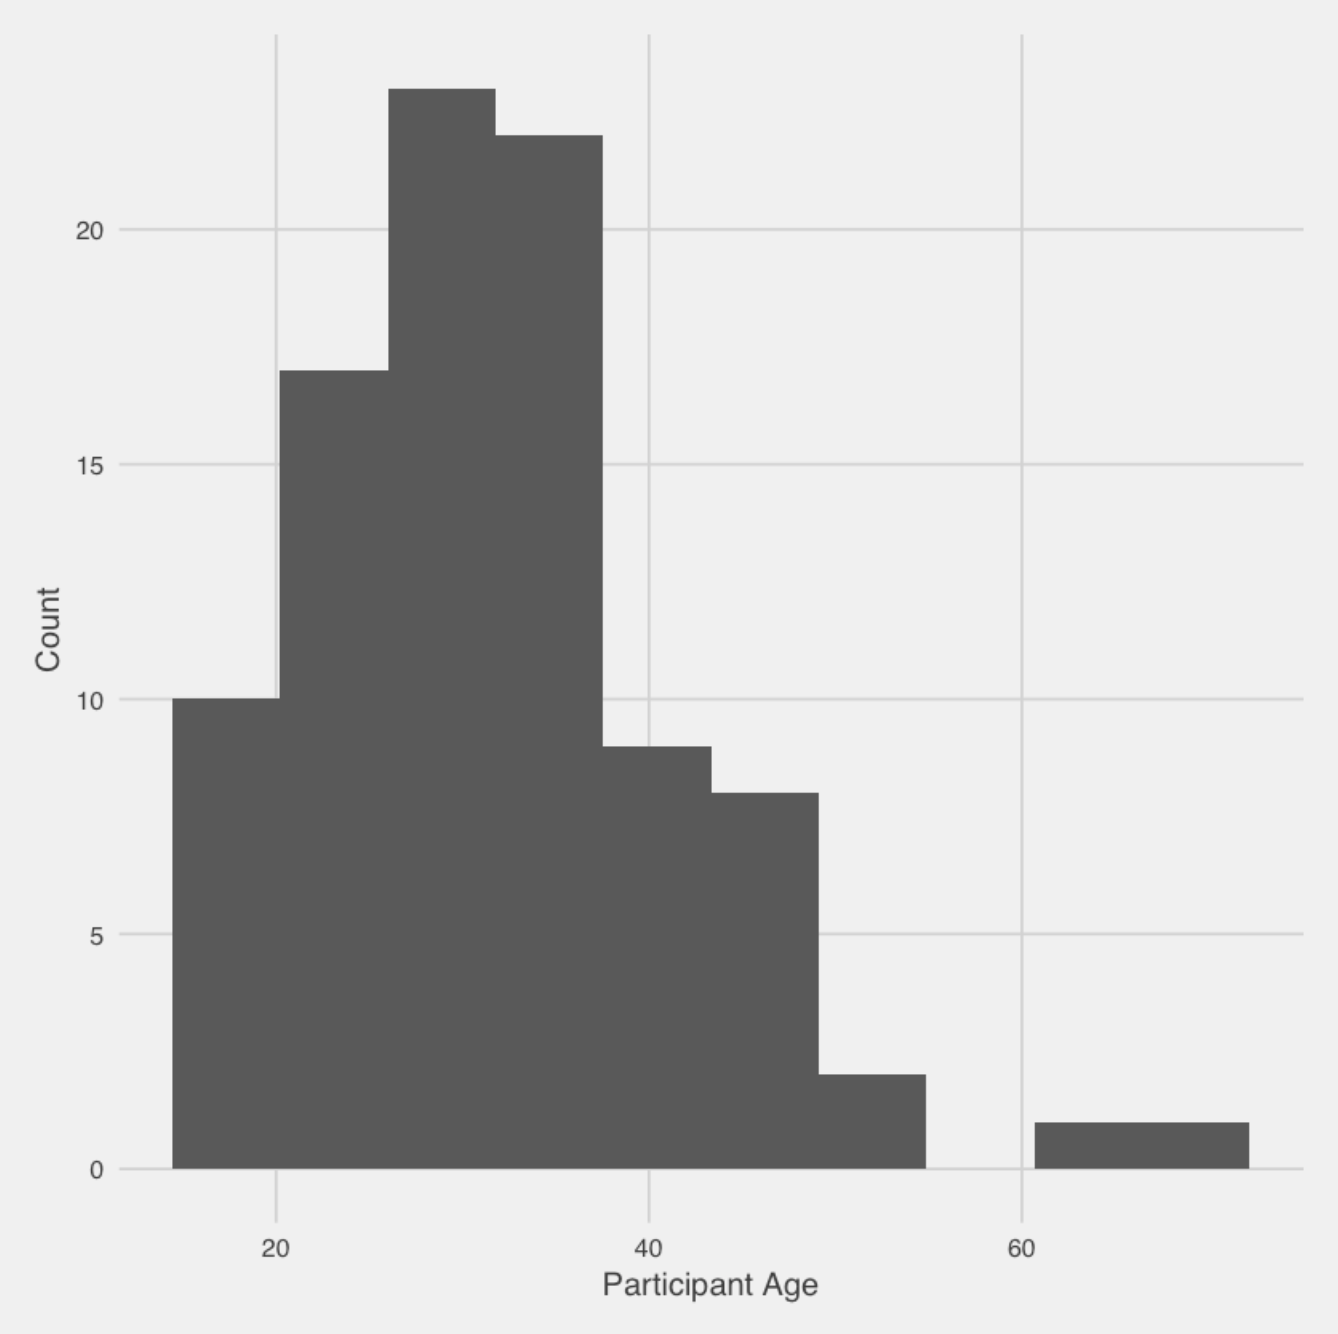
\includegraphics[width=.7\textwidth]{figures/age_distribution}
\caption{Distribution of participant ages}
\label{fig:age}
\end{figure}


\section{Procedure}

\subsection{Pre-Study Survey}

Recruitment materials directed participants to an initial survey, which was used to collect the demographic information reported above and information about how participants used their phones.

\subsubsection{Texting Use}
This study collects SMS data. This choice is in part pragmatic -- the Android SMS database is accessible via Android API's, and therefore any Android application can access this data. Other mobile messaging platforms are proprietary, and their message data could not be collected as easily, if at all. While the use of other mobile messaging apps is on the rise~\citep{duggan2015mobile}, SMS still remains a popular option~\citep{smith2015us}. 

Given that restrictions on texting, such as having a limited text plan, could influence the texting behavior of interest in the study, participants were asked if they were aware of any limits on their SMS plan. No participants reported having such limits.

While the focus of this study is on SMS, other messaging platforms such as Google Hangouts and Facebook Messenger are also popular. Participants were asked what other messaging applications they use, and how their use of SMS compared to the use of these other platforms. All participants reported using at least one other messaging application. Forty-six percent of participants said they used SMS more often than these other applications, and 28\% reported using SMS about the same amount as the other applications. Twenty-five percent said they use SMS somewhat less often than other messaging applications, with only 1\% reporting using SMS a lot less often.

\subsection{SMS Tracking Application}

After completing the pre-study survey, participants were emailed a link to a custom Android application developed to collect their text messages and experience sampling data when responding to messages. They were also provided with detailed instructions about the app and measures involved. Participants were required to run the app for 7 days, after which they were sent instructions on how to uninstall the app. After 7 days, the app was automatically disabled, so even if participants did not immediately uninstall the application, no further data was collected.

A background service monitored the SMS database on participants' Android phones, transmitting and storing all messages sent and received during the study period on an external database, managed by Northwestern School of Communication IT. All sensitive information, including phone numbers and message content, were encrypted before being sent to the Northwestern database. These encrypted values were also stored in the Northwestern database to help ensure participant privacy. Multimedia content, such as photographs and videos, were not stored in the Northwestern database, but indications that they were sent or received were transmitted and placeholders indicating their presence were saved in the Northwestern database. Given the focus of this study on dyadic interaction, only dyadic conversations were stored (i.e., not group texts).

\subsubsection{Session Initiation Attempts}

Although mobile owners text frequently throughout the day~\citep{battestini2010large}, the focus of this study is on how much the factors described above affect responsiveness to new conversations. These moments represent when a message sender likely has the least information available to them regarding the recipient's availability. In other words, once a recipient responds, the original message sender has received a response, he can assume the recipient is available to talk (or the recipient can explain that they are not currently available). With the goal of this project being to contribute to develop a better model of potential differences in sender and receiver attitudes towards responsiveness due to a mismatch in information, conversation initiations are a useful filter to apply to all messages sent to focus on when this mismatch is greatest. Following\citet{avrahami2006responsiveness}, I refer to messages from contacts that start a new conversation \textit{session initiation attempts} (SIA's). An SIA is any message that begins a new conversation session. \footnote{Once users are engaged in a texting conversation, they tend to respond quickly~\citep{battestini2010large}, whereas we would expect more variation in responsiveness in deciding whether or not to engage with a conversation initiation. This was also true in the data collected for this project, where responses to SIA messages had a median response time of a little over three minutes, whereas non-SIA messages had a median response time of 35 seconds.}

SIA's were identified using a heuristic similar to \citet{avrahami2006responsiveness}, where an SIA is any incoming message from a contact that is sent after some threshold has passed since the last interaction with that contact. The threshold chosen for this study was 30 minutes, which was selected after reviewing large scale studies of texting behavior~\citep{battestini2010large,birnholtz2017attending}, as well as discussion with pilot study participants. The focus of this study is solely on study participant responses to SIA's received from their contacts (i.e., not on SIA's by participants to their contacts).

To illustrate SIA's, refer to Figure~\ref{fig:sia}. Grey text bubbles represent a participant and blue text bubbles represent a contact they text with. The incoming message that starts ``Hey, I don't want to wait...'' would be considered an SIA because it comes from the contact, and at least 30 minutes have passed since the last time the participant texted that contact. The message ``So like 1 or 2'' is also an SIA since it has been more than 30 minutes since the last  message ``Early afternoon'' was sent. However, the ``Okay I'll be ready at 2'' messages would not be considered an SIA since only 10 minutes have passed since the last time the participant texted the contact. 
 
The determination of whether or not a message is an SIA is based on the messages preceding it, but both messages from the participant and from the contact are used in making this determination. In Figure~\ref{fig:sia}, ``What time do you want to leave?'' is an SIA because it has been longer than 30 minutes since the participant texted the contact. In Figure~\ref{fig:sia2}, ``Where are yas?'' is an SIA because it has been 43 minutes since the last time the contact last texted the participant.

A potential issue with this heuristic approach is that it ignores ``follow up'' texts. Imagine, for example, that the session initiator in Figure~\ref{fig:sia} followed up their 12:56pm ``What time do you want to leave'' text with a 1:00pm text that just said ``??'', a technique that has been observed to heighten attention from a contact~\citep{heston2017worth}. In this case, we are still interested in responsiveness as it related to the initial 12:56pm text. To deal with this, if a message was registered as an SIA, any follow up texts were grouped with that initial text, with the timestamp of the SIA being associated with the original text.

\begin{figure}[h]
\centering
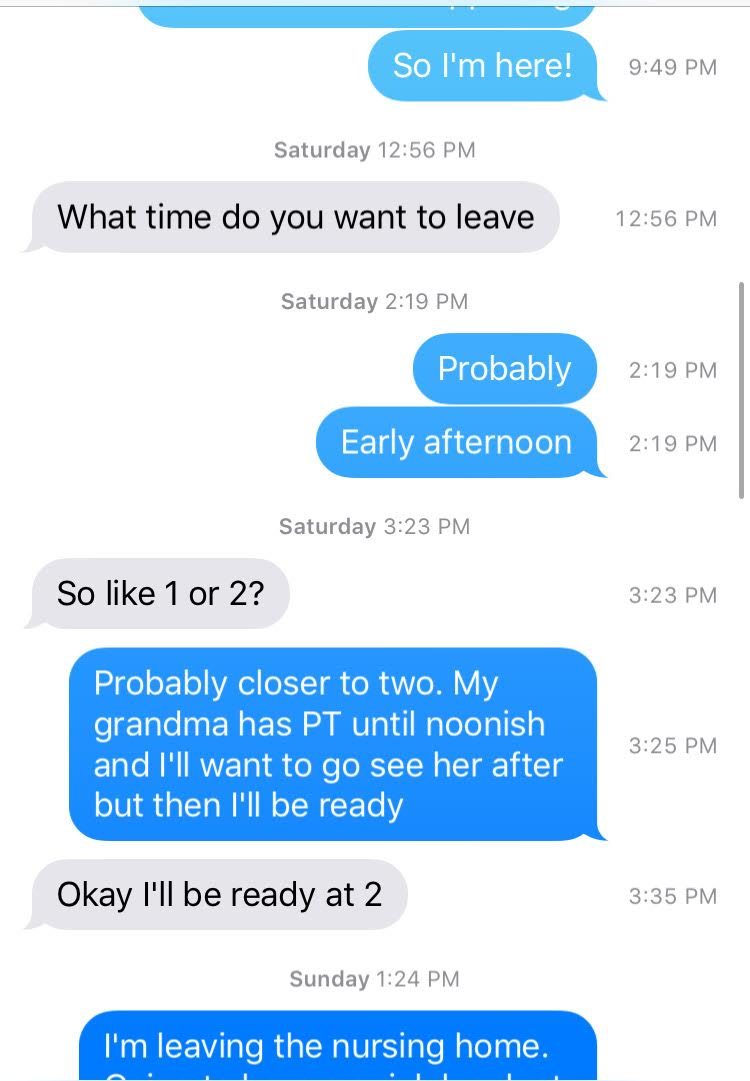
\includegraphics[width=.7\textwidth]{figures/example_sia}
\caption{Example text message exchange}
\label{fig:sia}
\end{figure}

\begin{figure}[h]
\centering
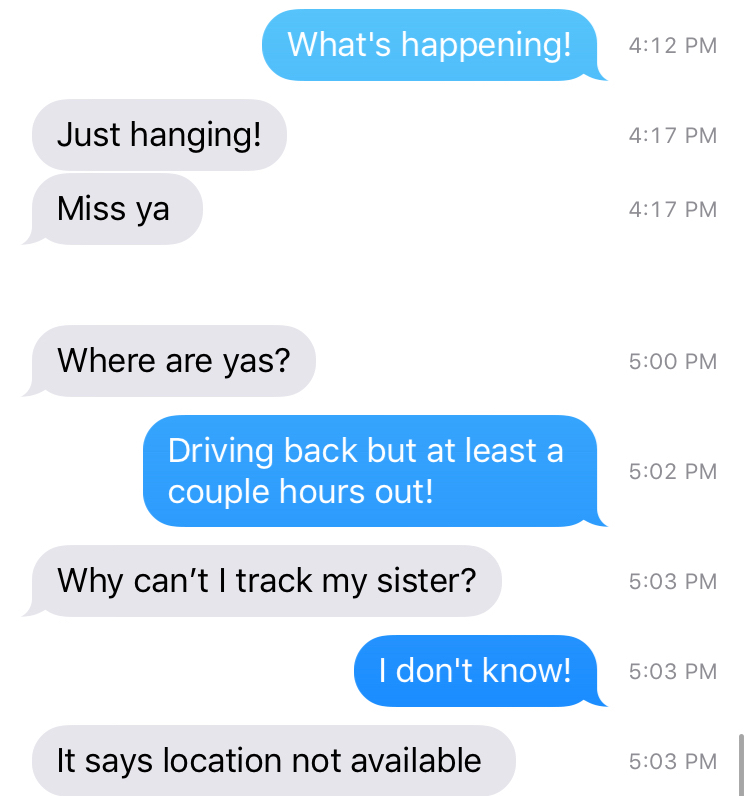
\includegraphics[width=.7\textwidth]{figures/sia2}
\caption{Example text message exchange}
\label{fig:sia2}
\end{figure}


\subsubsection{Experience Sampling}
\label{sec:esm}

Whenever a participant responded to an SIA, they would receive a notification on their phone to fill out a short questionnaire about the message they were responding to, following an event-based approach to experience sampling method (ESM)~\citep{conner2009experience,csikszentmihalyi2014validity}. It is normally recommended experience sampling  be triggered immediately at the moment of interest~\citep{hormuth1986sampling}, e.g., in this case, participants could be asked about text message the moment it is received, rather than when they respond to it, removing the need for a retrospective answer. However, this could have other consequences which affect study validity. Our primary variable of interest is response time. Sending the user multiple notifications about an incoming message (i.e., both the notification for a message and the notification asking for their availability), could cause the participant to behave differently than they otherwise would, e.g., responding to the message when they otherwise wouldn't, since they are responding to our prompt anyway. In addition, notifying immediately after response ensures the notification is received at a time participants are on their phones and able to answer the questionnaire.

It is important to note that, as a result of this decision, this study focuses only on SIA's that received a response during the study period. If an SIA was never responded to, no data about it could be collected. In other words, results should be interpreted as factors that affect how quickly a user responds in the case where a message eventually receives a response, not if a user ever decides to respond at all.

It should also be noted that SIA's were identified using a heuristic, and like any heuristic, it could at times be inaccurate. Consider, for example, a case where a participant texts a contact ``Goodnight'' at the end of the day. The contact doesn't see the message until an hour later, but still responds ``Goodnight.'' The following morning, the participant texts the contact ``Are we still on for lunch today?'' The app would consider this a response to an SIA, because since over 30 minutes has passed since they last sent a message, the contact's ``Goodnight'' would be considered an SIA. But including this in the dataset is inaccurate, since the participants morning message is not a response to the ``Goodnight'' message. To deal with these cases, participants were able to dismiss the ESM questionnaire by saying the message they just sent was not a response to to the received message. To ensure participants understood what messages the prompt referred to, they were shown timestamped copies of the message they just sent and what it was being recorded as a response to.

After reviewing the message they just sent, the contact they sent it to, the initial SIA they were responding to, and the time that SIA was received. They were then asked to rate the following items:

\textbf{Availability.} Participants first declared themselves as unavailable or available. If they were available, they then rated their availability on a 1--5 scale, with lower values indicating being busy or distracted and higher values indicating not being busy at all. In the results presented below, these values were collapsed into a 0-6 scale, where 0 indicates the participant having marked themselves as unavailable.

Other responsiveness studies have used sensor data, such as phone activity, to make inferences about availability, rather than using ESM to collect this directly~\citep[e.g.,][]{pielot2014didn}. However, such studies focus only on predicting responsiveness, rather than making inferences about responsiveness behavior. Given the focus of this work on understanding how different variables affect responsiveness, capturing an availability measure directly should allow for better inference in how message content and sender-receiver relationship interact with a participant's own subjective feeling of availability.

The distribution of availability across collected SIA's are shown in Figure~\ref{fig:availability_distribution}.

\begin{figure}[h]
\centering
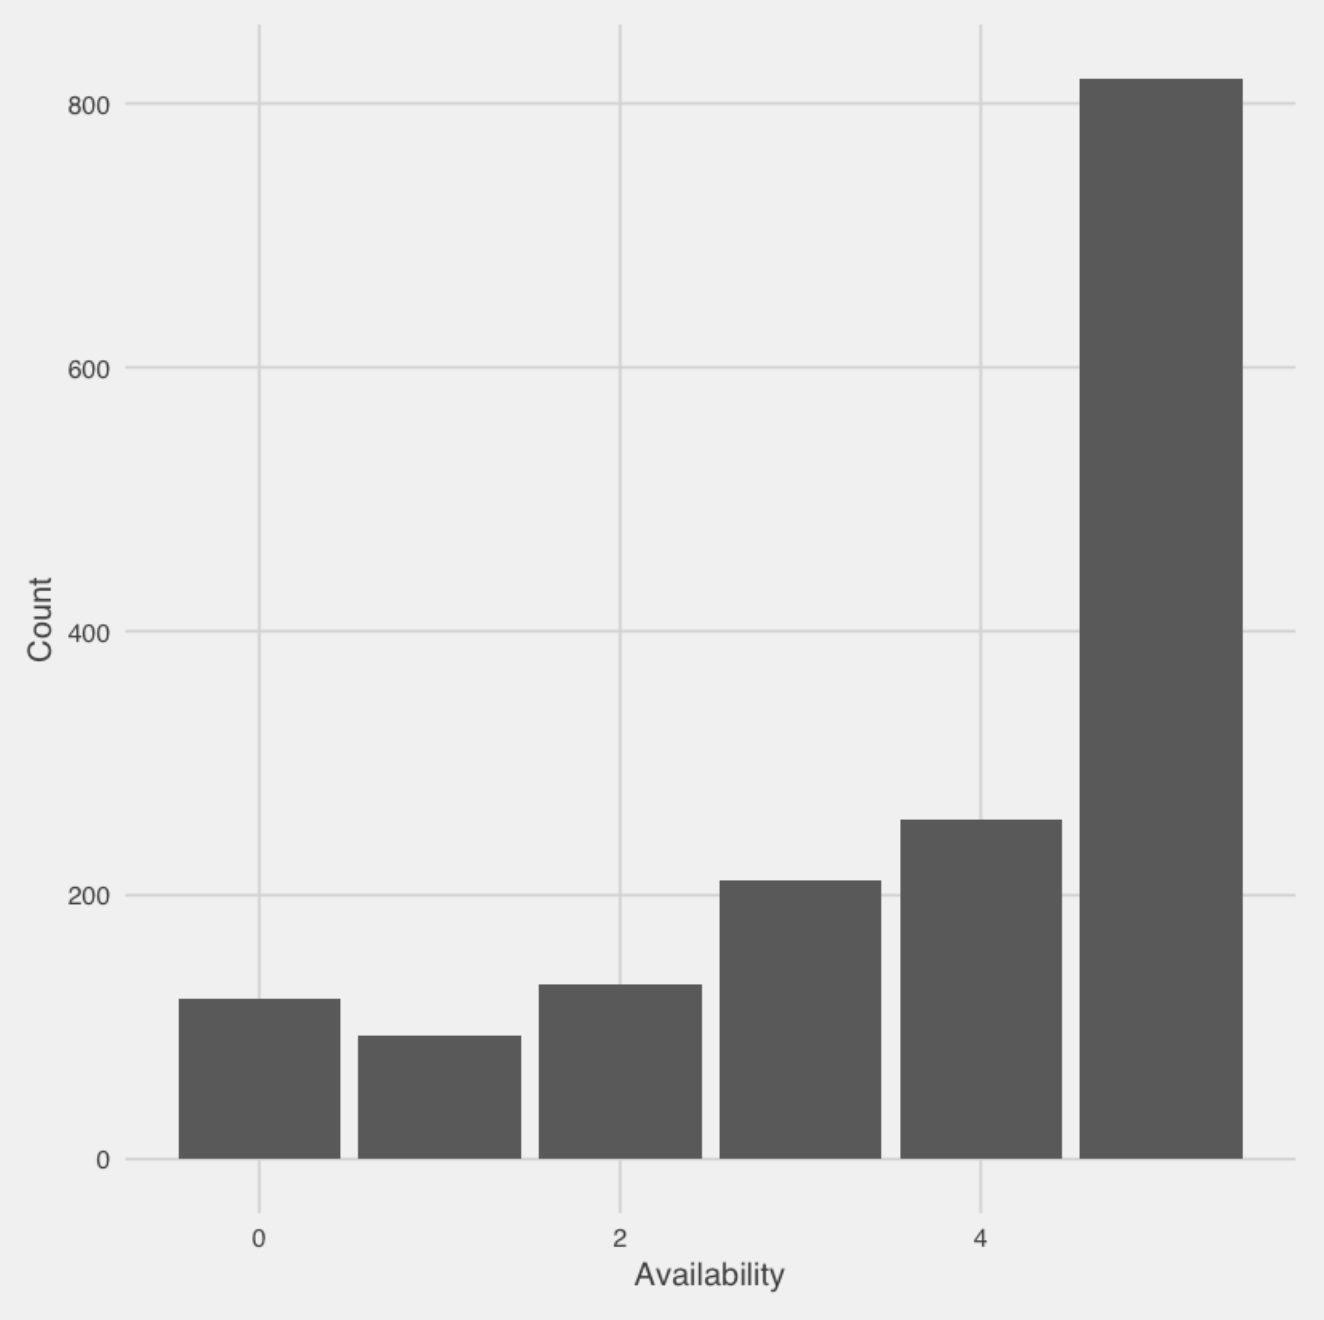
\includegraphics[width=.7\textwidth]{figures/availability_distribution}
\caption{Distribution of availability for SIA messages.}
\label{fig:availability_distribution}
\end{figure}


\textbf{Message Importance.} Participants rated each SIA on a 1--5 ``How important is this message to you?'' scale (referred to in results as ``importance to contact''). The distribution of this measure is shown in Figure~\ref{fig:importance_distribution}.

\begin{figure}[h]
\centering
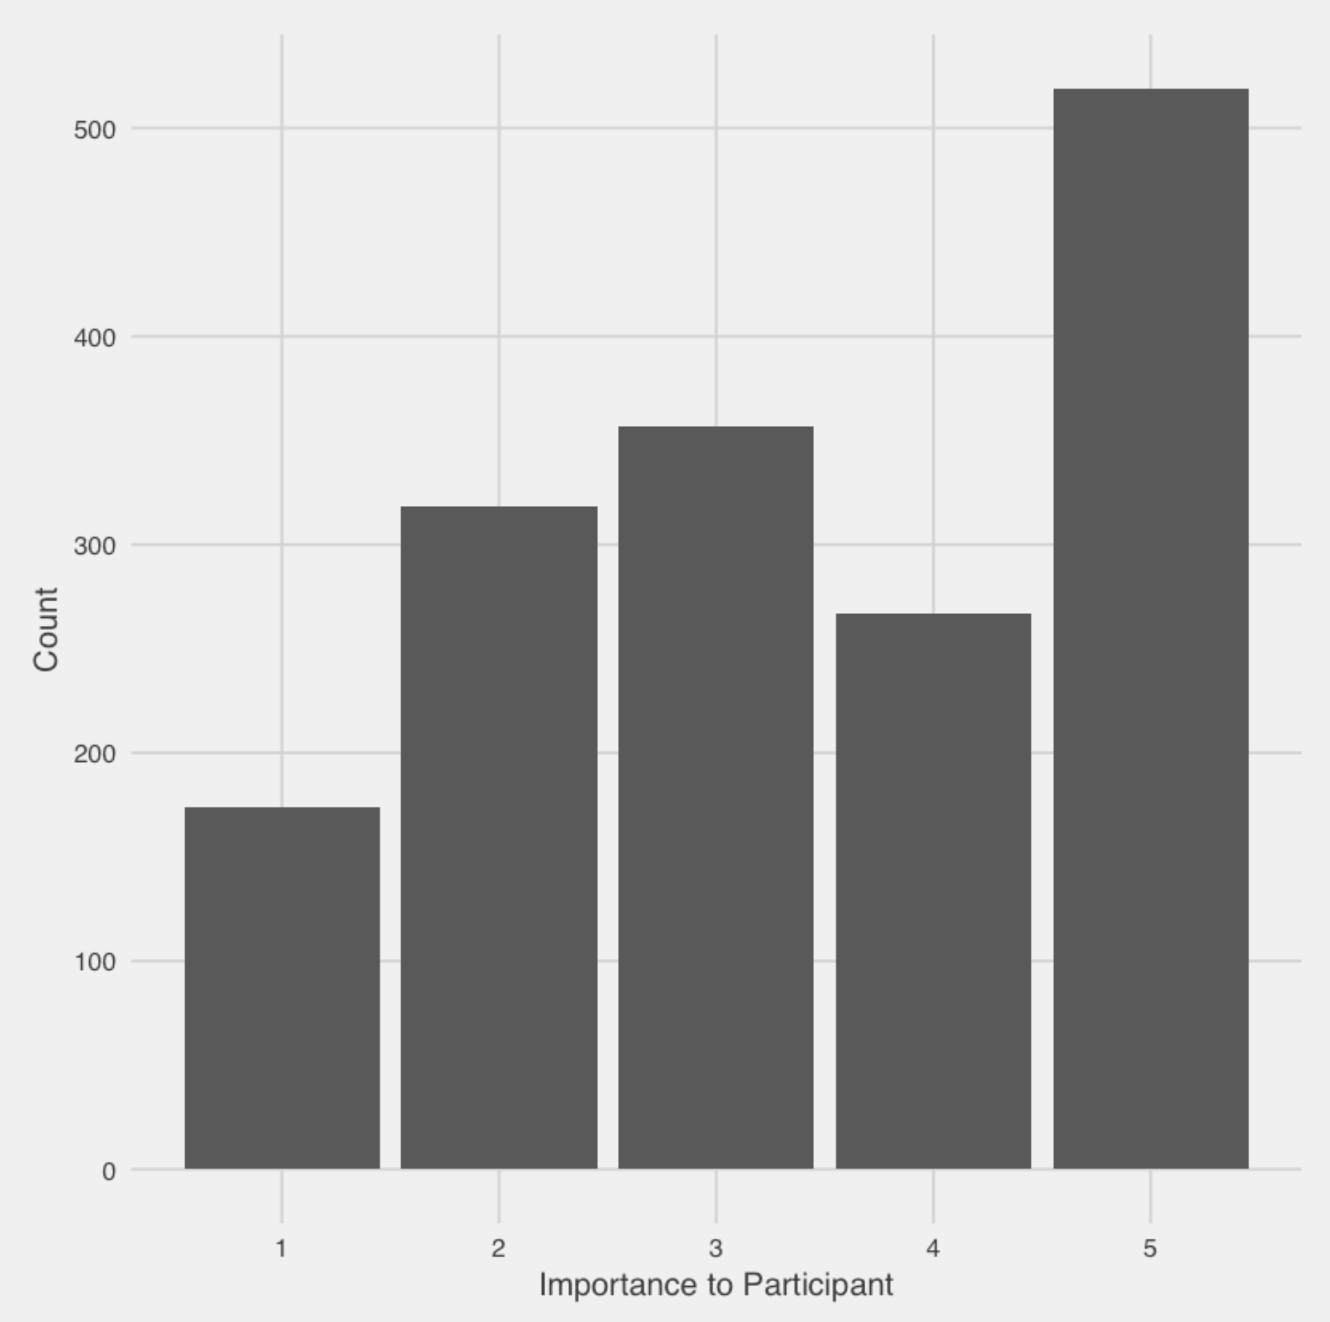
\includegraphics[width=.7\textwidth]{figures/importance_distribution}
\caption{Distribution of importance to participant for SIA messages.}
\label{fig:importance_distribution}
\end{figure}

Participants also rated each message on a 1--5 ``How important do you think this message is to the person who sent it to you?'' (referred to in results as ``importance to contact''). Distribution of this measure is shown in Figure~\ref{fig:importance_contact_distribution}.

\begin{figure}[h]
\centering
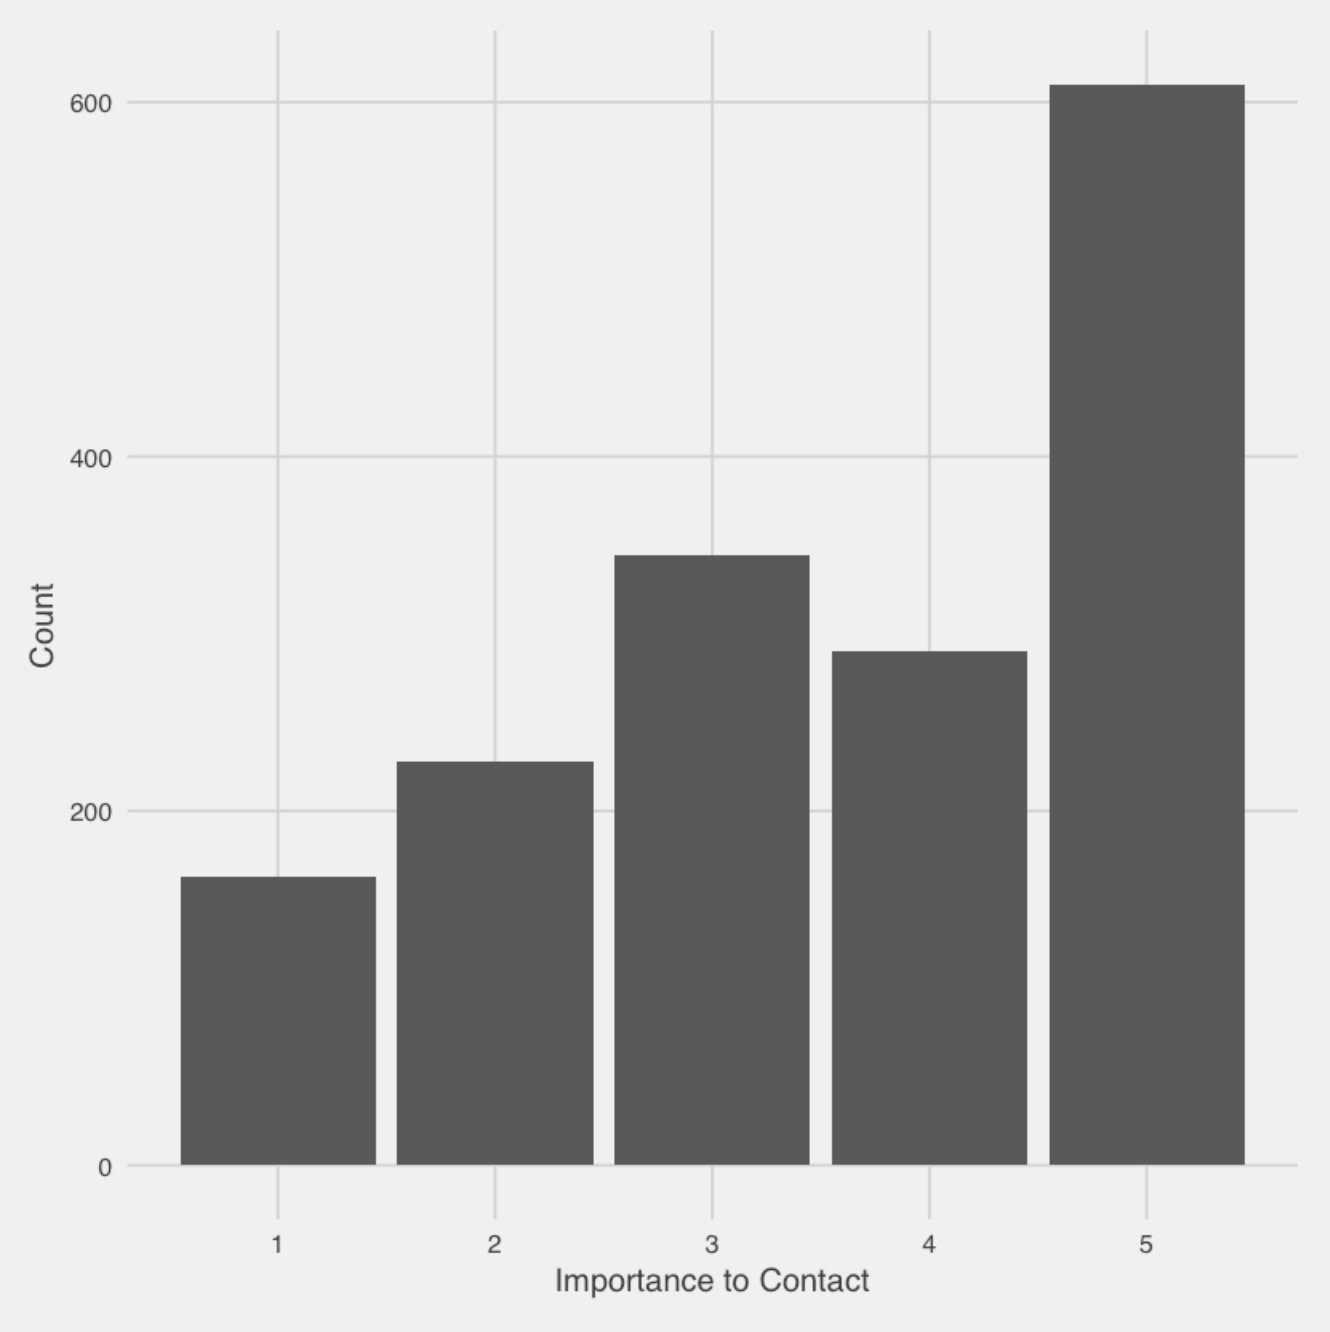
\includegraphics[width=.7\textwidth]{figures/importance_contact_distribution}
\caption{Distribution of importance to contact for SIA messages.}
\label{fig:importance_contact_distribution}
\end{figure}


\subsection{Post-Study Survey}

After running the SMS tracking application for 7 days, participants were sent a final survey where they rated each of their contacts who sent them an SIA during the study on 2 relational scales. Intimacy was measured using a 3 item scale adapted from \citet{miller1982assessment}. Power was measured using a 3 item scale adapted from \citet{farrell2015relationship}. The distribution of these variables across contacts are shown in Figures \ref{fig:intimacy} and \ref{fig:power}. Higher levels on the intimacy scale refer to feeling closer to that contact and higher values on the power scale indicate the contact has more power over the participant.  To account for potential differences in texting behavior based on the proximity of the message sender to the message receiver (e.g., a person may have different texting habits with someone who lives in their same city that they see often versus a friend who lives in a different state who they see rarely), for each contact, participants also specified proximity from one of the following options: ``We live together,'' ``In the same city, but we don't live together,'' ``In the same state, but not the same city,'' ``In the same timezone, but not the same state,'' ''In a different time zone.'' The distribution of the proximity measure is shown in Figure~\ref{fig:proximity}.


\begin{figure}[h]
\centering
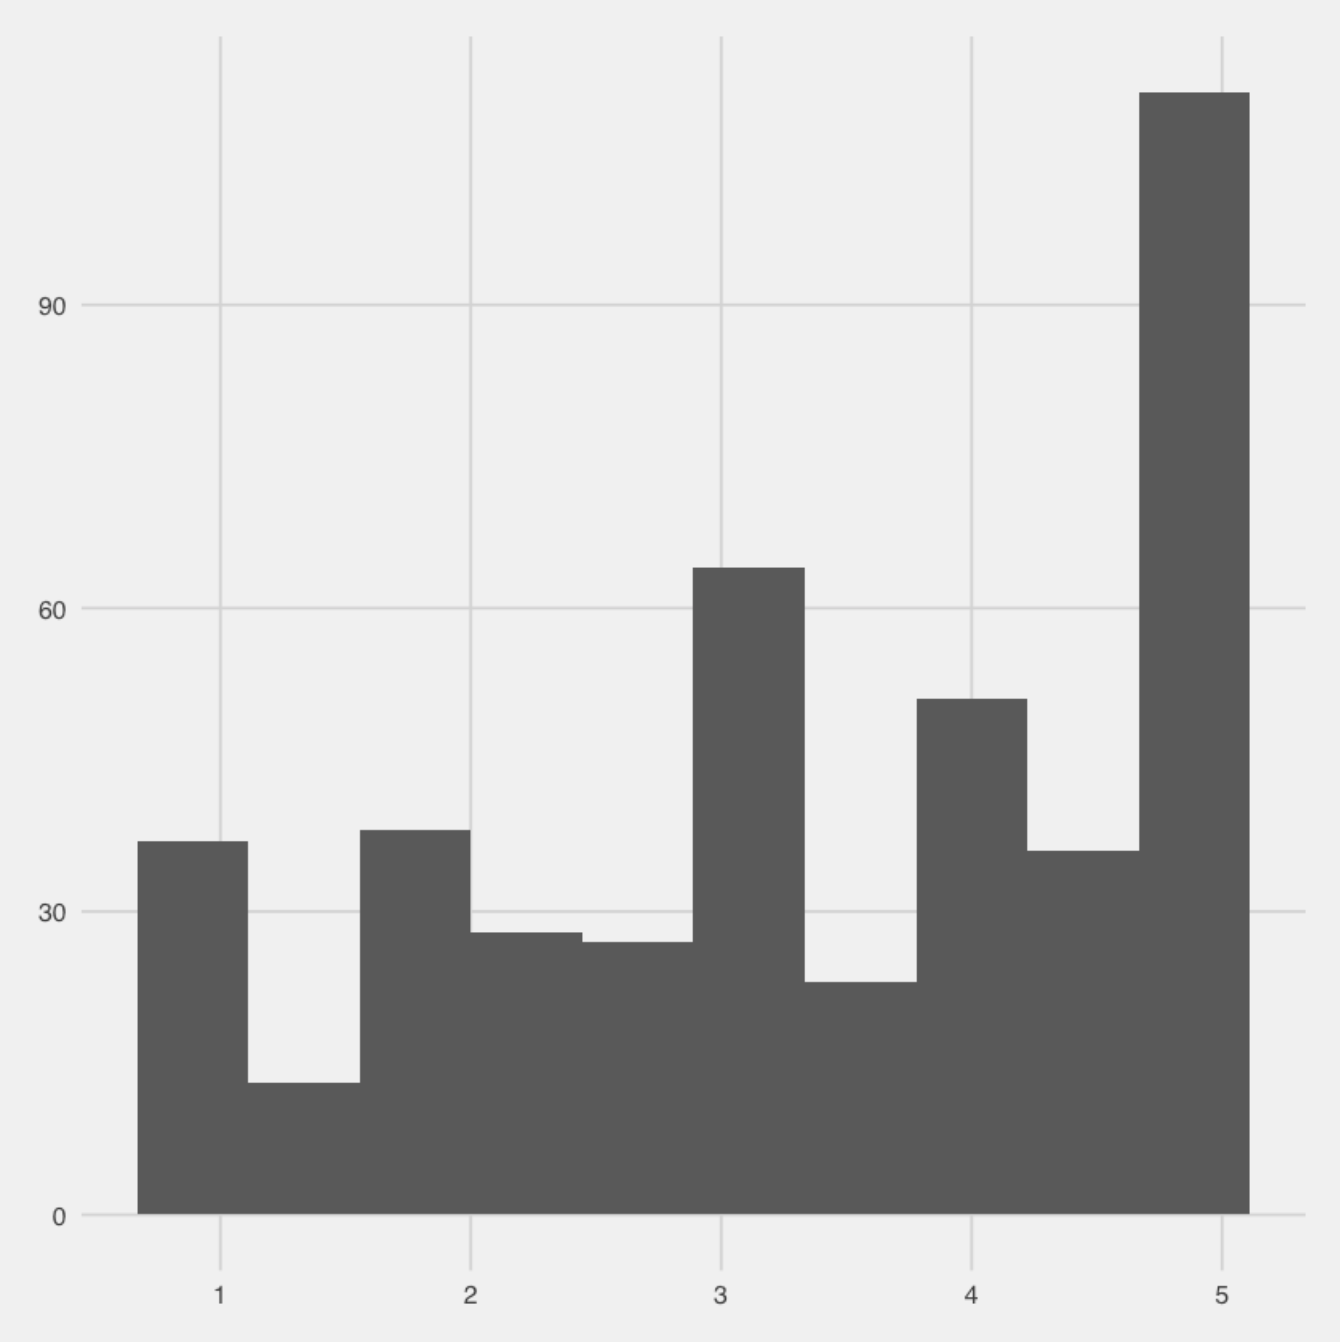
\includegraphics[width=.7\textwidth]{figures/intimacy_distribution}
\caption{Distribution of measured intimacy across contacts.}
\label{fig:intimacy}
\end{figure}


\begin{figure}[h]
\centering
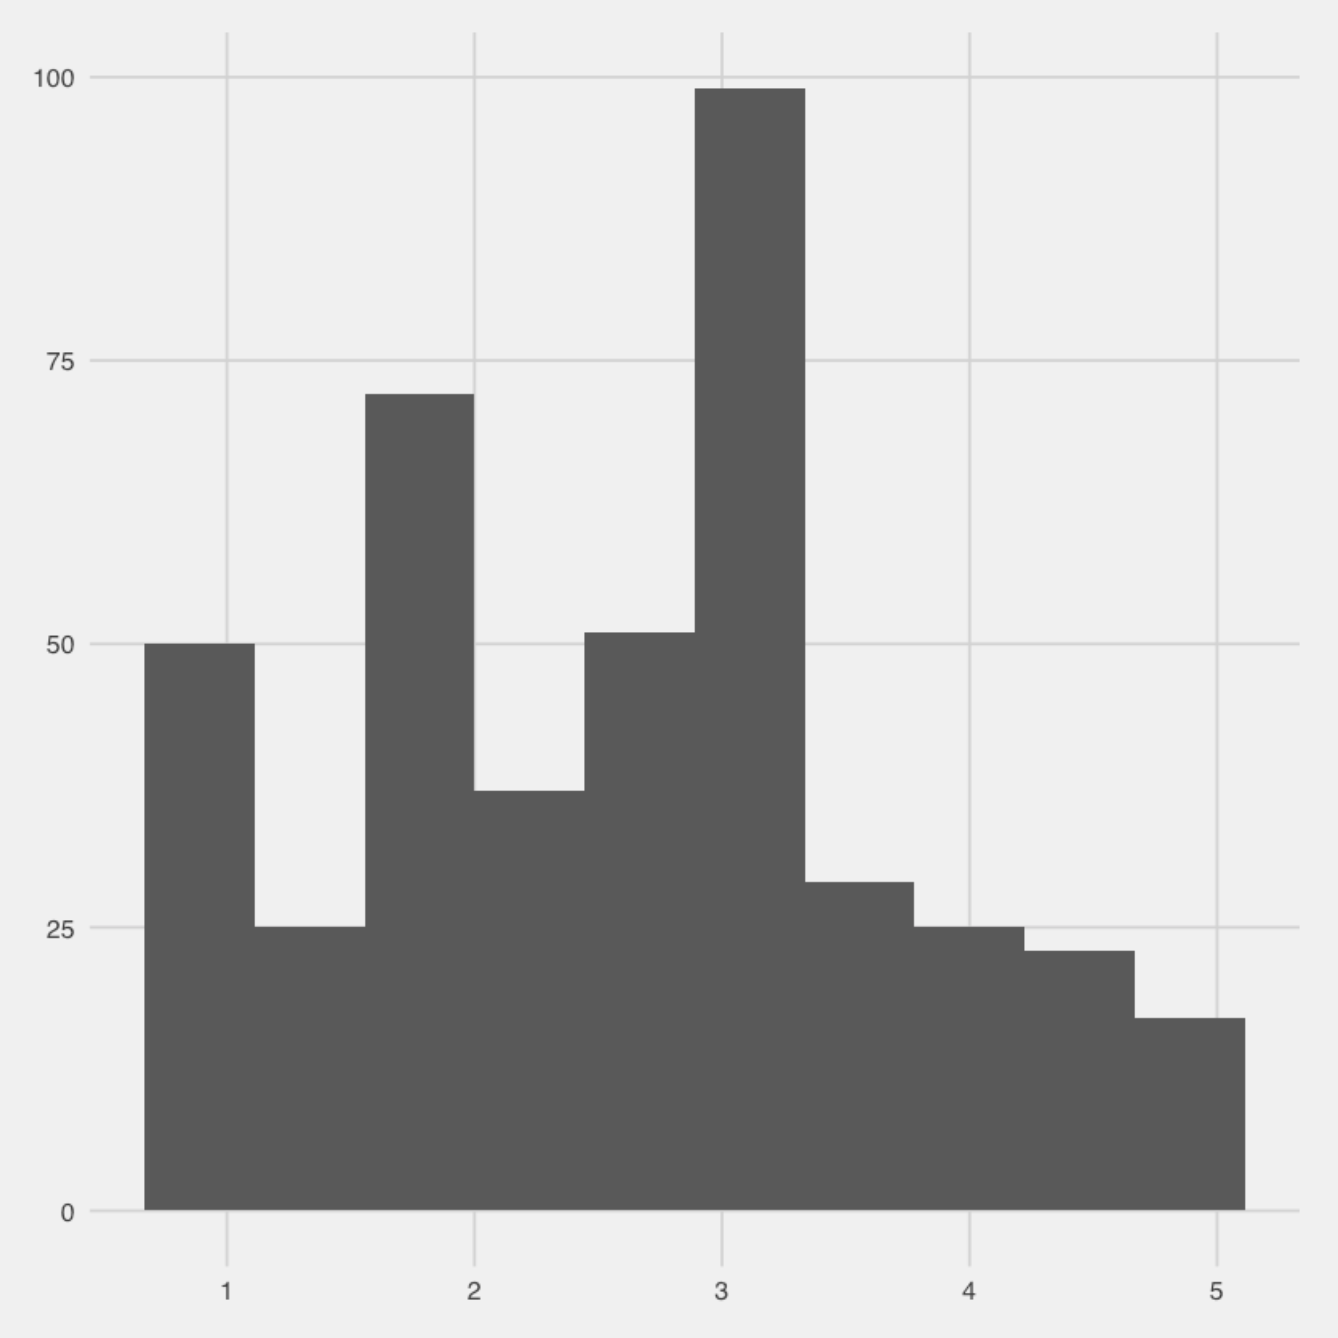
\includegraphics[width=.7\textwidth]{figures/power_distribution}
\caption{Distribution of measured power across contacts.}
\label{fig:power}
\end{figure}

\begin{figure}[h]
\centering
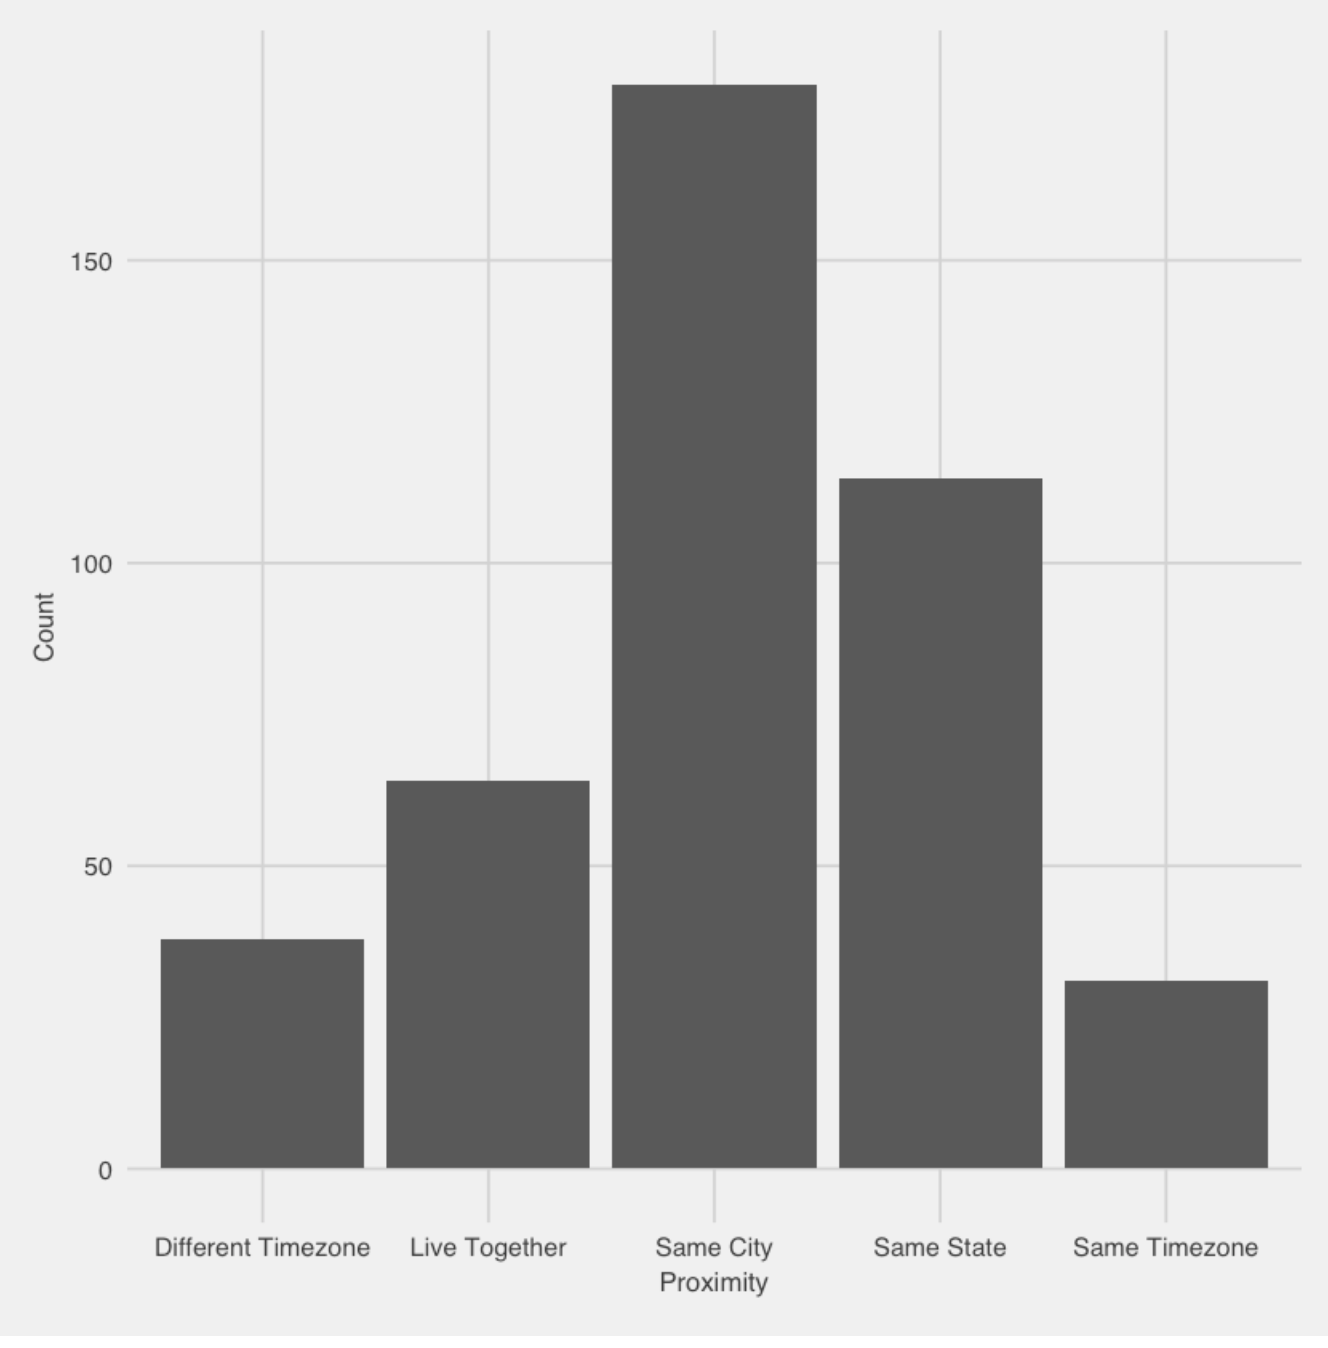
\includegraphics[width=.7\textwidth]{figures/proximity_distribution}
\caption{Distribution of proximity across contacts.}
\label{fig:proximity}
\end{figure}


\subsection{Post-Study Content Coding}

After data collection, SIA messages were manually coded as either non-requests, information requests, or action requests. Development of these codes was based in part on the distinction by \citet{cui2016beyond} in a qualitative study of mobile messages between ``spontaneous interaction,'' which includes general information exchange and emotional communication, and ``purposive communication,'' which includes coordination and assistance. The decision to further reduce requests into information requests and action requests follows a coding scheme by \citet{dabbish2005understanding} in a study of email responsiveness, where each had different effects on responsiveness behavior. These codes are explained in Table~\ref{tab:codes}.

\begin{table}[]
\centering

\begin{tabular}{lp{6cm}p{5cm}}
\hline
Code                & Definition                                                                                                                             & Example                                                                                          \\ \hline
Non-request         & Greeting, expressing mood or sharing experience. Any comment showing engagement but not explicitly asking anything from the recipient. & "I’ll be home tomorrow I love you," "I got the pictures developed."                              \\
Information Request & Coordinating activity, problem solving, or any explicit request that can be fulfilled by responding to the text message.               & "Where you at dog?," "Where did you want to go?"                                                 \\
Action Request      & Request where fulfillment requires non-texting action.                                                                                 & "See if mom left the container out," "When you go upstairs, see if the security guard is there." \\ \hline
\end{tabular}
\caption{Message type codes.}
\label{tab:codes}
\end{table}

All SIA messages were coded by the author. To ensure coding validity, a secondary coder was trained on the codebook and coded a sample of 20\% of messages. Inter-rater reliability as measured by Krippendorf's alpha was 0.74. A majority of messages (72\%) were non-requests, 22\% were information requests, and 6\% were action requests.

%Section~\ref{sec:esm} discussed how participants rated each message on 2 1--5 scales assessing message importance. In addition to these subjective assessments of messages, there is some evidence that different types of messages also influence responsiveness behavior.

%Early work on CMC tended to broadly discuss messages as either social or task-oriented~\citep[e.g.,][]{addas2015many,dabbish2005understanding,walther1992interpersonal}, which could in turn affect responsiveness. \citet{dabbish2005understanding}, for example, found that social messages typically were responded to more slowly than task-oriented messages.

%However, these studies focused on workplace CMC platforms. The notion of ``task-based'' is likely different there than it is in mobile messaging, where users are messaging with a more diverse set of contacts about different topics, rather than work-related projects. Nevertheless, social vs. task-based does provide one useful way of thinking about messages in that it describes a schemata that distinguishes messages that are requesting something from a recipient vs. those that are not.

%A useful framework is provided by \citet{cui2016beyond}, whose qualitative study content coding mobile messages broadly defines messages as ``spontaneous interaction'' vs. ``purposive communication.'' Spontaneous interaction captures messages whose purpose was primarily just checking in with a contact, where purposive communication had a more clearly defined purpose, such as coordinating an activity. \citet{cui2016beyond} also found differences in response time to these messages, where coordination messages received faster responses.

%To account for how message type might affect responsiveness behavior, content coding of all SIA messages received by participants was performed following data collection. All messages that could be considered ``spontaneous interaction'' were coded as ``non-requests.'' ``Purposive communication'' messages were further broken down into ``information requests'' and ``action requests''. Information requests were any message that explicitly asked for information which could be received over text message (e.g., ``What time do you get off work tonight?''). Action requests explicitly required action from the participant, which could not be fulfilled by simply responding to the message (e.g., ``Can you pick up milk on your way home?'').

%The focus on request types rather than the labels ``spontaneous'' vs. ``purposive'' used by ~\citeauthor{cui2016beyond} is due to that his study interviewed mobile messaging users and his labels could refer to the intent behind their message. In contrast, there is no way to know the true purpose of why a contact of a participant sent a message must necessarily focus on what is explicitly shown in the message. Furthermore, distinguishing requests as either information requests or action requests follows a coding scheme by \citet{dabbish2005understanding}. Although this work did not focus on mobile messaging, it did find significant differences between these types of requests in email.

%Mobile messaging users have reported feeling the need to respond to certain types of messages faster, such as those requesting help with a task~\citep{cui2016beyond}. Following content coding used in \citet{dabbish2005understanding}, messages were coded as either not a request, an action request (asking someone for some offline action, e.g., ``Can you pick up milk on your way home?'') or an information request (e.g., ``What time do you get off work tonight?'') A majority of messages (72\%) were non-requests, 22\% were information requests, and 6\% were action requests.

\section{Analysis}

Given the hierarchical nature of the collected data, data was analyzed using a series of multilevel models~\citep{gelman2007data}, with SIA's grouped within contacts grouped within participants.

In all regression models, the dependent variable was the natural log of the seconds in response latency between the receipt of an SIA and the response. The distribution of response time in seconds, shown in Figure~\ref{fig:response_time}, is highly skewed, which is typical of response time distributions~\citep{kalman2006pauses}. Taking the log of this variable results in a more normal distribution, as shown in Figure~\ref{fig:log_response_time}. Other approaches to dealing with this type of skewed data include different classes of generalized linear models~\citep[see e.g.,][]{buntin2004too,dick2004beyond,manning2001estimating}, but experimentation with these models demonstrated poor model fit for the collected data.

To understand the impact of how different classes of independent variables (i.e., message attributes and relational variables) affect responsiveness, a hierarchical regression process was followed wherein a series of regression models were fit introducing a new class of variables at each step~\citep{gurnsey2017statistics}. To test whether or not variables improved model fit, likelihood ratio tests were used to compare models. In addition to these tests, model fit parameters such as the Akaike information criterion (AIC) were compared, as suggested by \citet{gelman2007data}.

\begin{figure}[h]
\centering
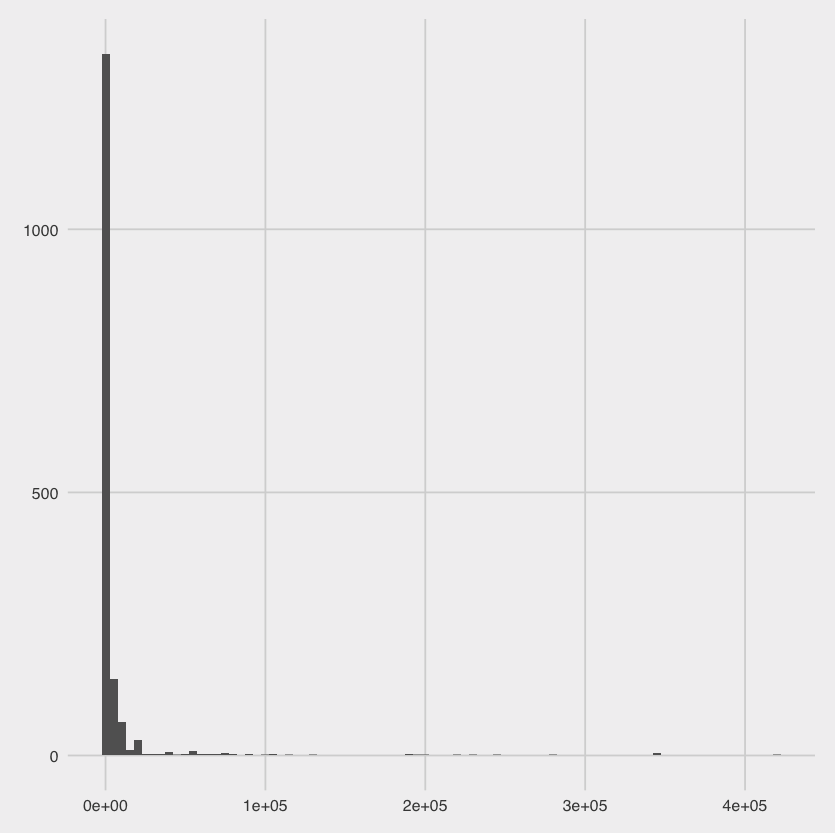
\includegraphics[width=.7\textwidth]{figures/response_time_distribution}
\caption{Distribution of response time in seconds.}
\label{fig:response_time}
\end{figure}

\begin{figure}[h]
\centering
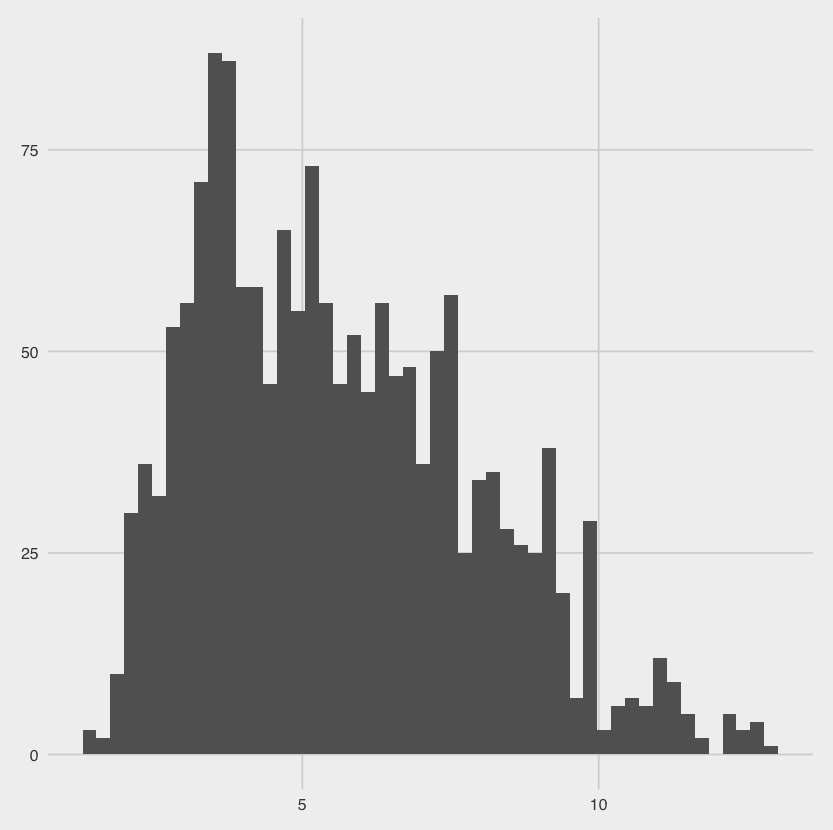
\includegraphics[width=.7\textwidth]{figures/log_response_time_distribution}
\caption{Distribution of the natural log of response time in seconds.}
\label{fig:log_response_time}
\end{figure}

\chapter{Results}

\section{Descriptive Statistics}

\subsection{General Texting Behavior}
\label{sec:texting}

The 92 participants who completed the study sent and received a total of 21,818 messages across 1,285 different contacts. About 50\% (10,941) of those were messages received by participants. The distribution of number of messages received over the 7-day study period across participants is shown in Figure~\ref{fig:received_messages}. The median number of received messages over the study period was 68.5. 

\begin{figure}[h]
\centering
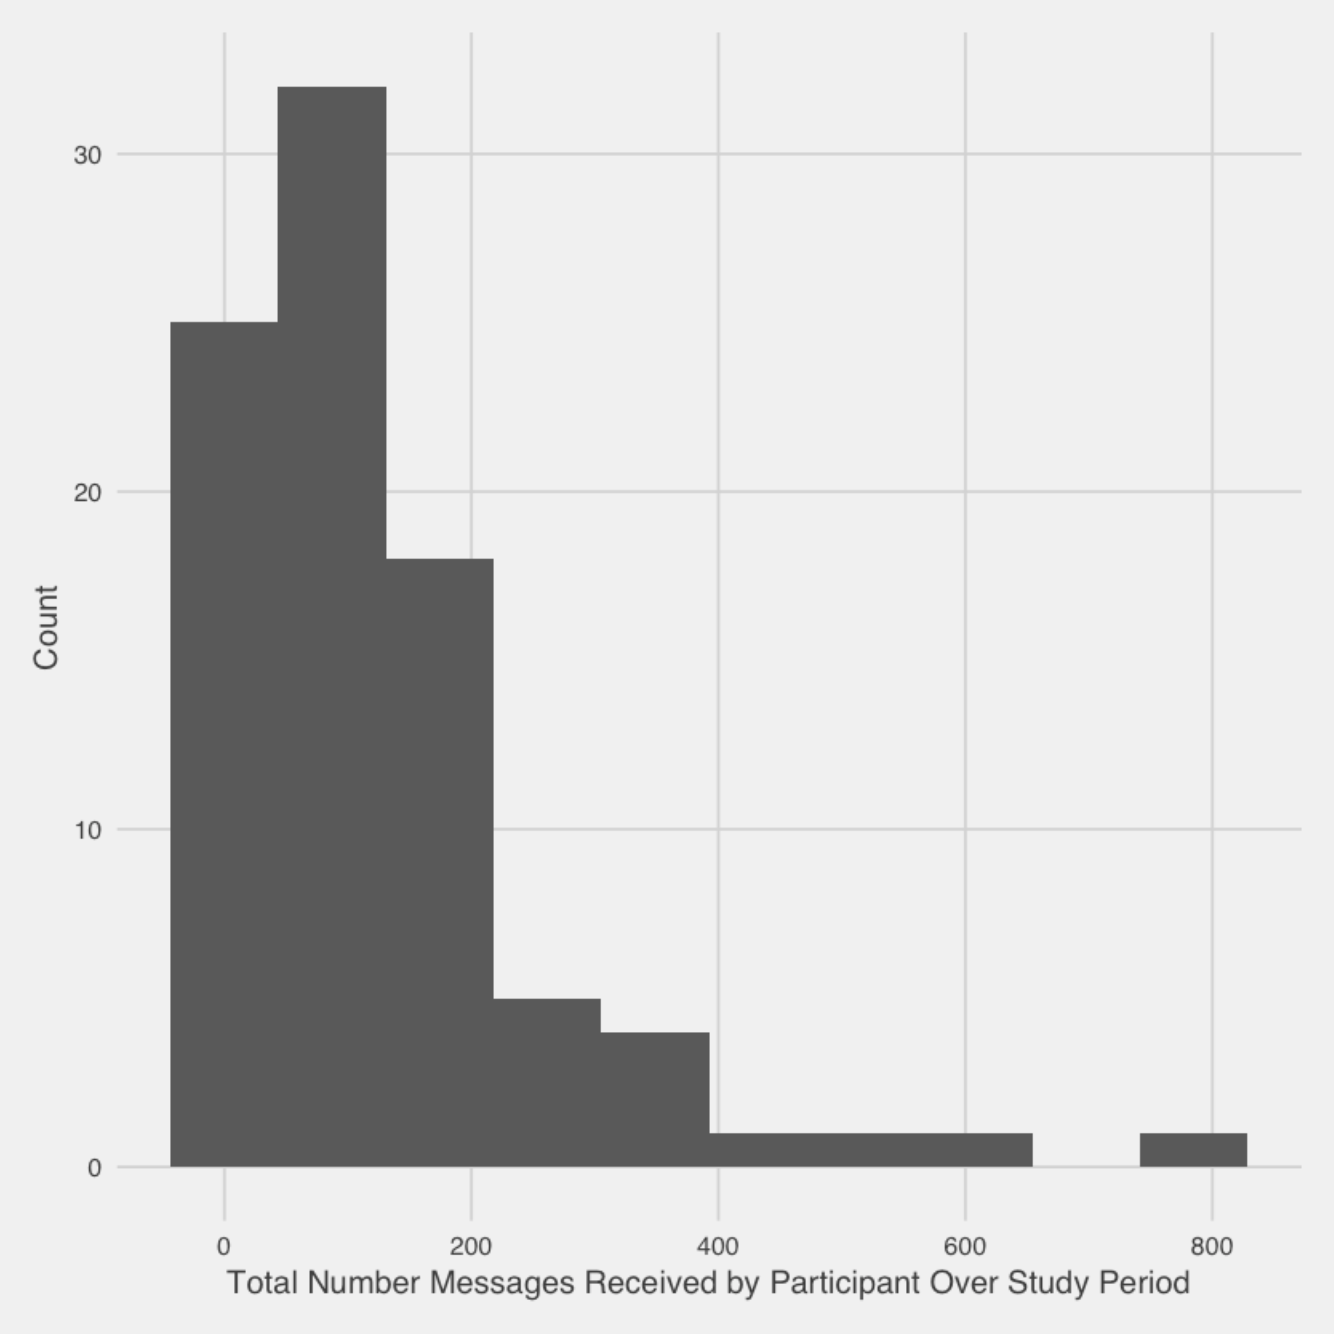
\includegraphics[width=.7\textwidth]{figures/all_messages_received_distribution}
\caption{Distribution of number of messages received over 7 day study period across participants.}
\label{fig:received_messages}
\end{figure}

The median number of contacts that participants texted with over the 7 day study period was 12. This distribution is shown in Figure~\ref{fig:num_contacts}. As seen in Figure~\ref{fig:received_messages_by_contact}, a large number of messages were received from a small number of contacts, with the distribution of messages received across contacts being highly skewed.

\begin{figure}[h]
\centering
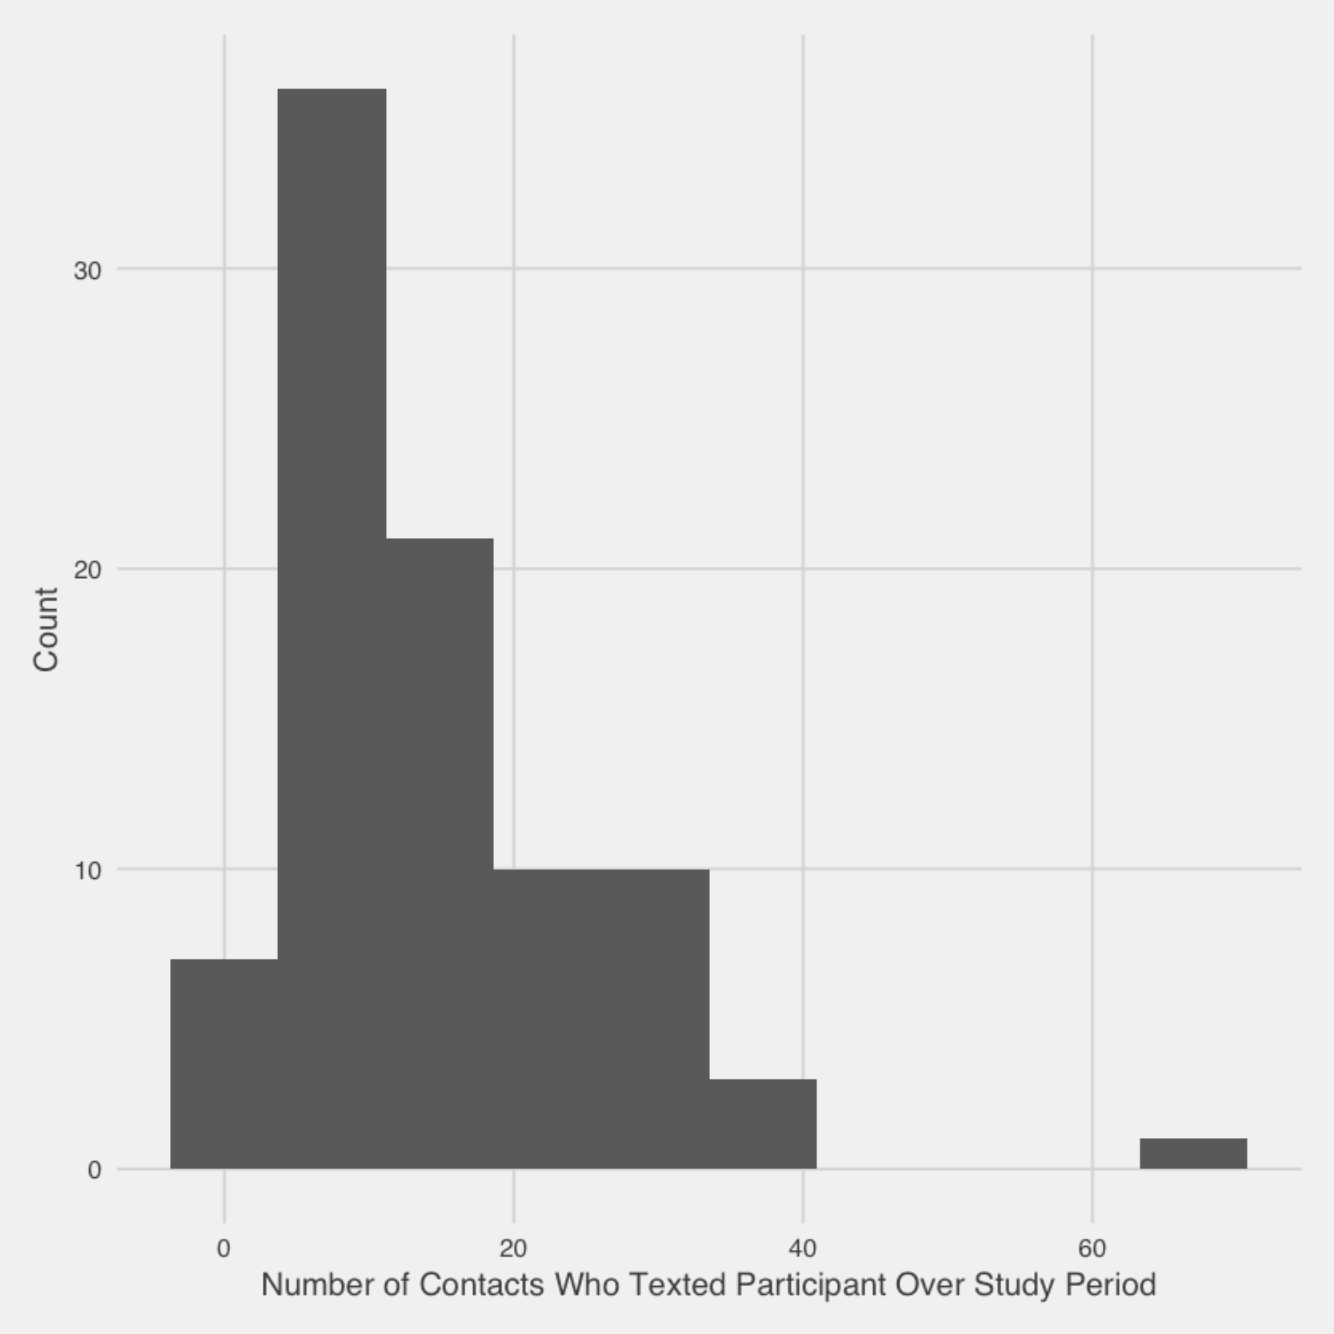
\includegraphics[width=.7\textwidth]{figures/all_messages_contacts_distribution}
\caption{Distribution of number of contacts communicated with over 7 day study period across participants.}
\label{fig:num_contacts}
\end{figure}

\begin{figure}[h]
\centering
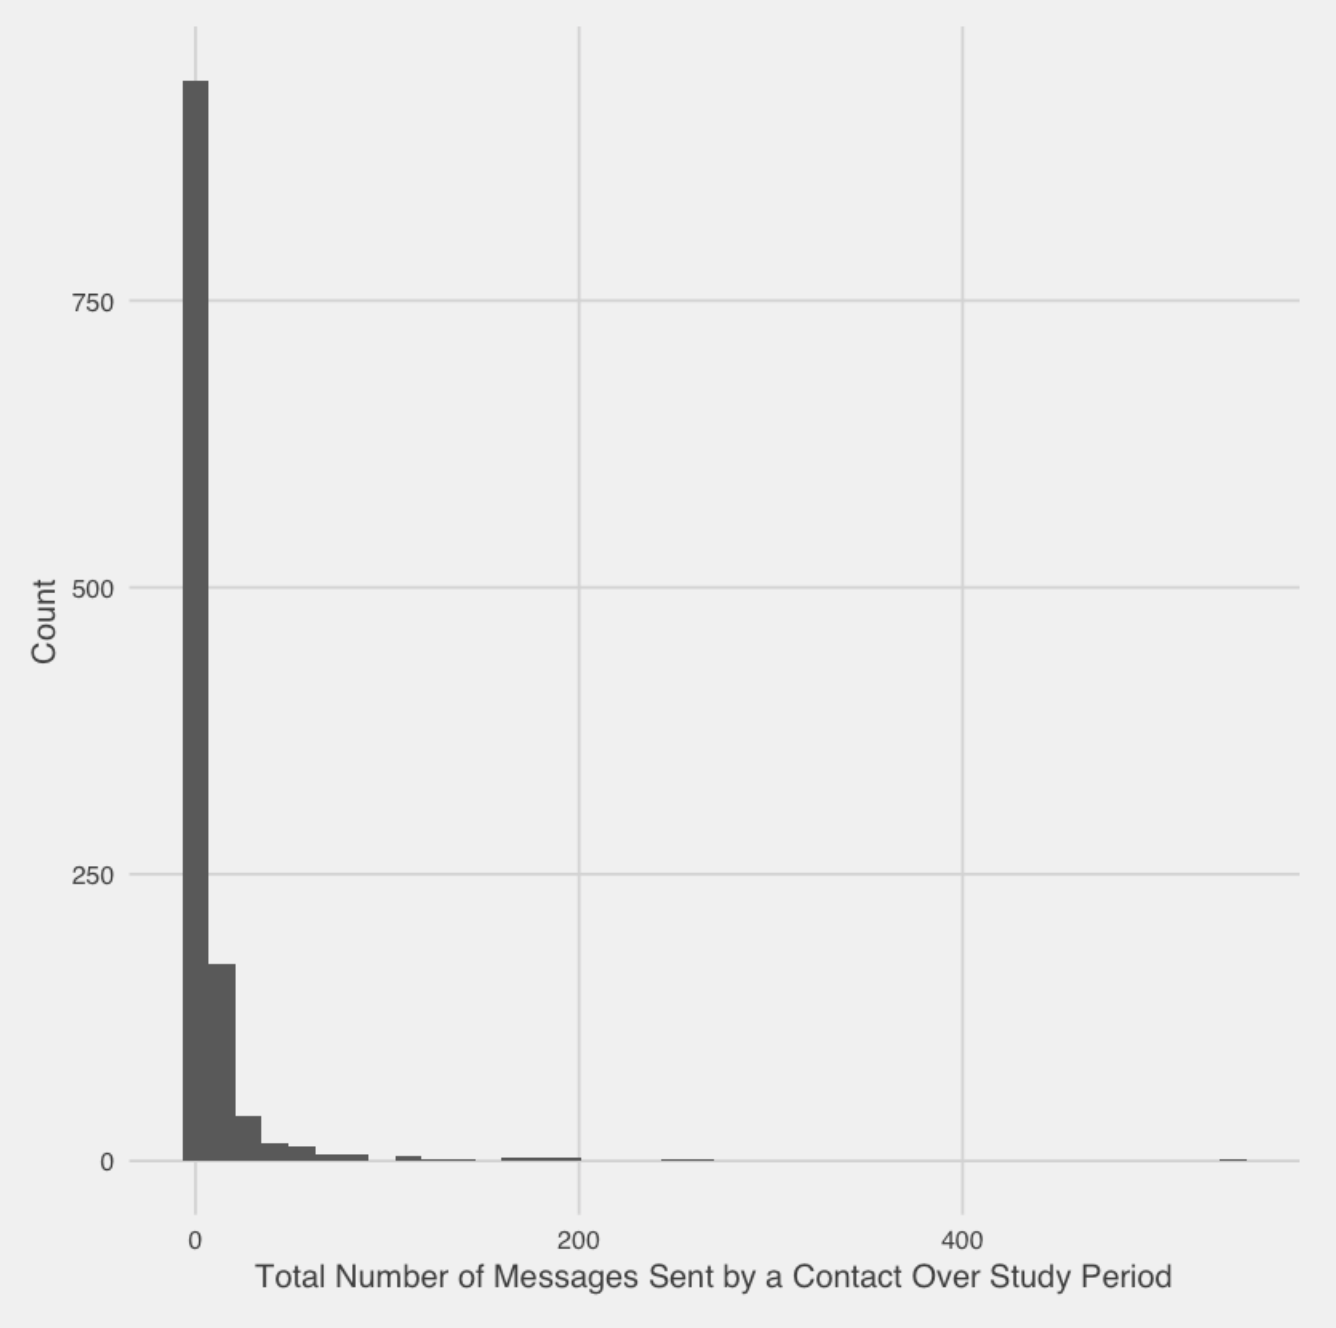
\includegraphics[width=.7\textwidth]{figures/messages_received_by_contact_distribution}
\caption{Distribution of number of messages received over 7 day study period across contacts.}
\label{fig:received_messages_by_contact}
\end{figure}


\subsection{Session Initiation Attempts}

Of the 10,491 received messages, 1,635 were identified as SIA's. The median number of SIA's received by a participant over the study period was 12, which followed a similarly skewed pattern as the number of total received messages (see Figure~\ref{fig:received_sia_messages}).

\begin{figure}[h]
\centering
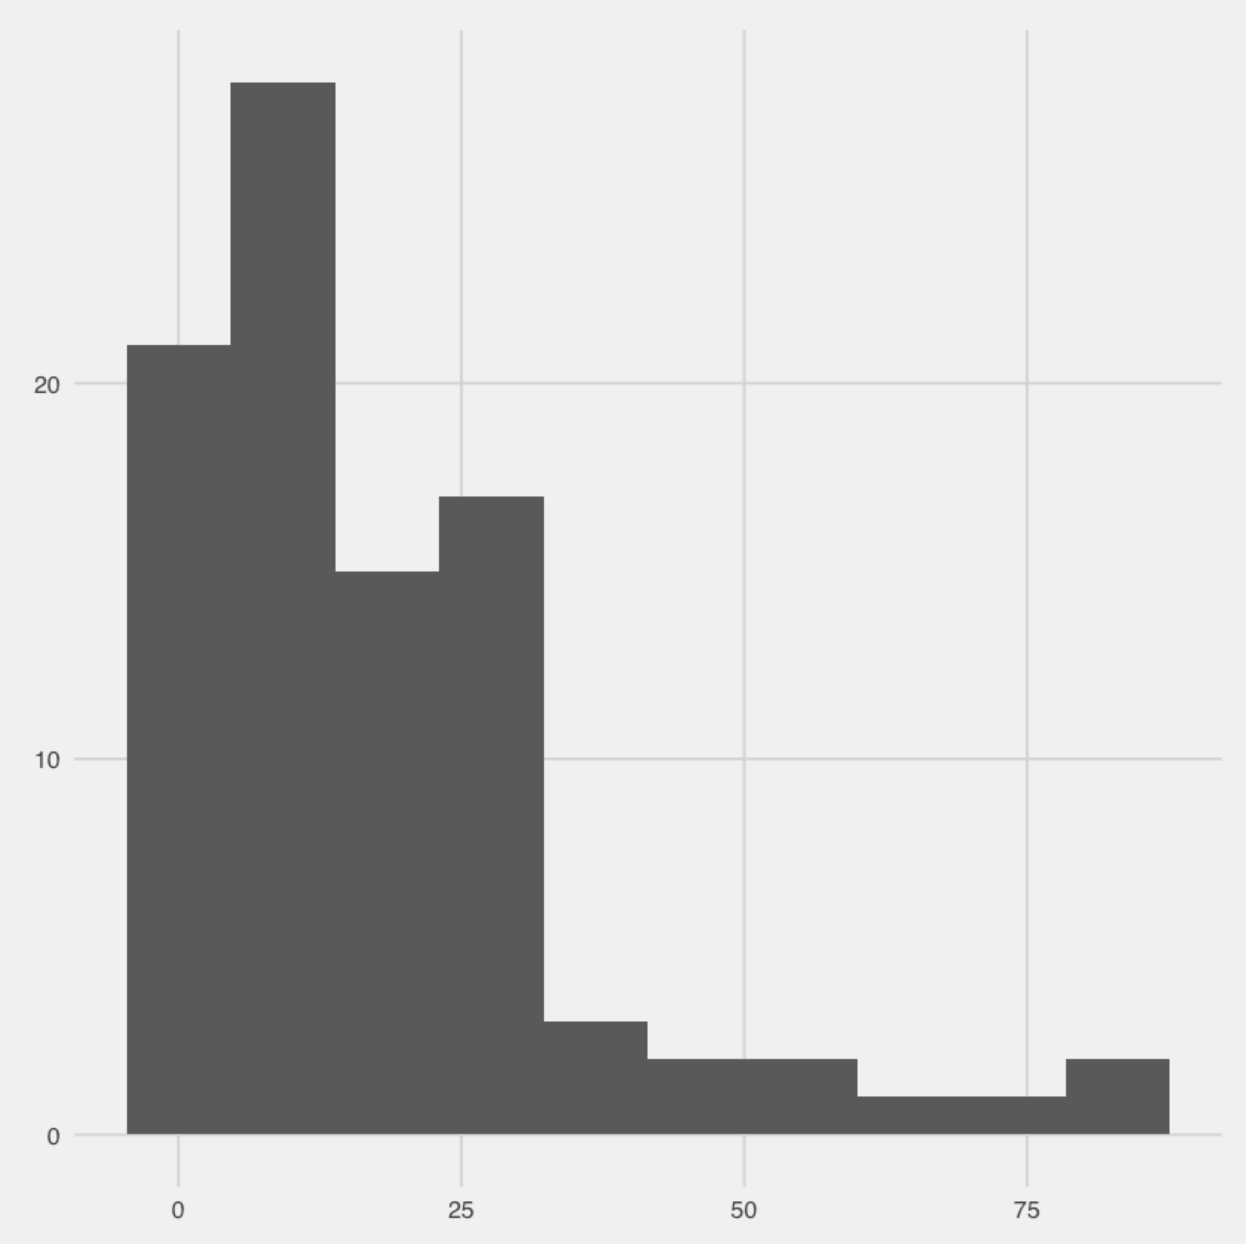
\includegraphics[width=.7\textwidth]{figures/sia_received_distribution}
\caption{Distribution of number of SIA messages received over 7 day study period across participants.}
\label{fig:received_sia_messages}
\end{figure}

SIA's came from a much smaller subset of contacts. Of the 1,285 contacts present in the total dataset, only 426 appear in the SIA data. The median number of contacts who sent a participant an SIA over the study period was 4 (see Figure~\ref{fig:sia_num_contacts}). The large difference in the number of contacts when considering all messages versus only SIA's can be explained in part by the skew seen in Figure~\ref{fig:received_messages_by_contact}. Of the 1,285 contacts represented in the dataset, 527 sent participants only 1 message. If a participant sent a contact a message, and then got a reply, and then they never communicated again during the study period, then they would not appear in the SIA data. If a participant received one message from a contact and never responded, they would also not appear in the SIA data. Furthermore, it is likely that some amount of ``contacts'' present in all messages do not represent true contacts and messages that would receive a response. For example, receiving a login code from a website via SMS would appear in the data shown in Section~\ref{sec:texting}, but not in SIA data.

\begin{figure}[h]
\centering
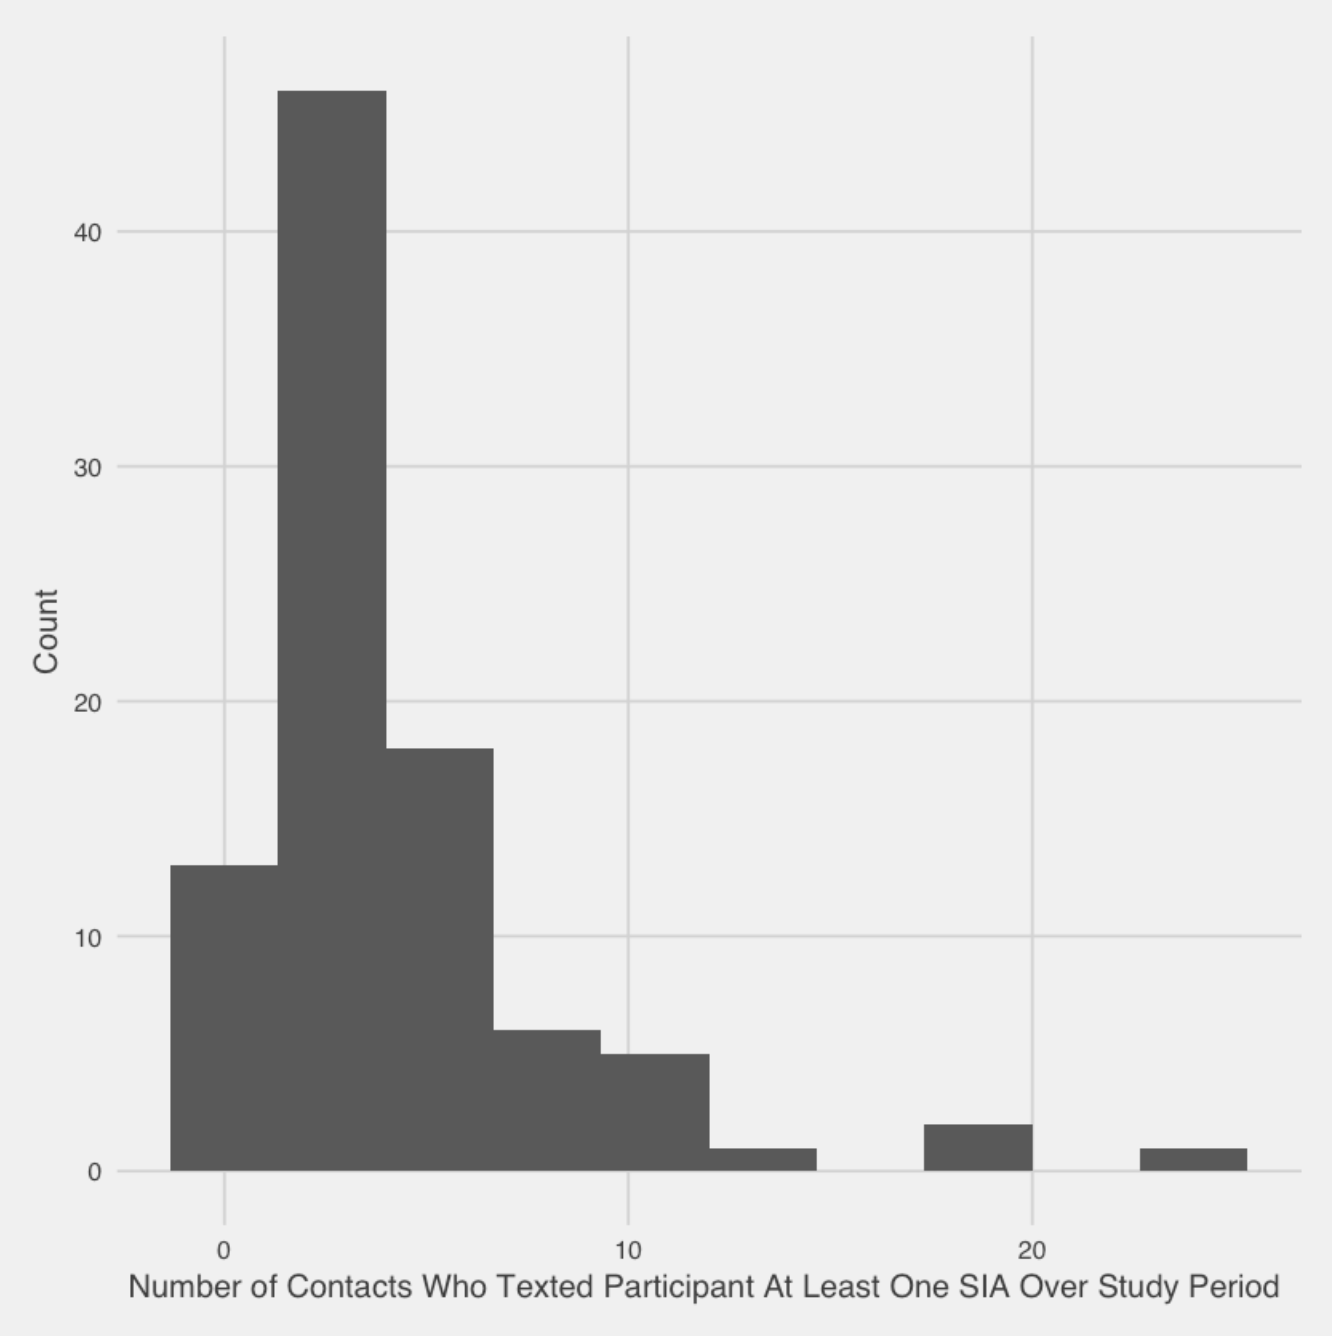
\includegraphics[width=.7\textwidth]{figures/sia_messages_contacts_distribution}
\caption{Distribution of number of contacts who sent SIA's with over 7 day study period across participants.}
\label{fig:sia_num_contacts}
\end{figure}

To demonstrate when SIA messages were received by participants, Figure~\ref{fig:sia_heatmap} displays a heat map showing the days of the week and the time of day SIA's were received.

\begin{figure}[h]
\centering
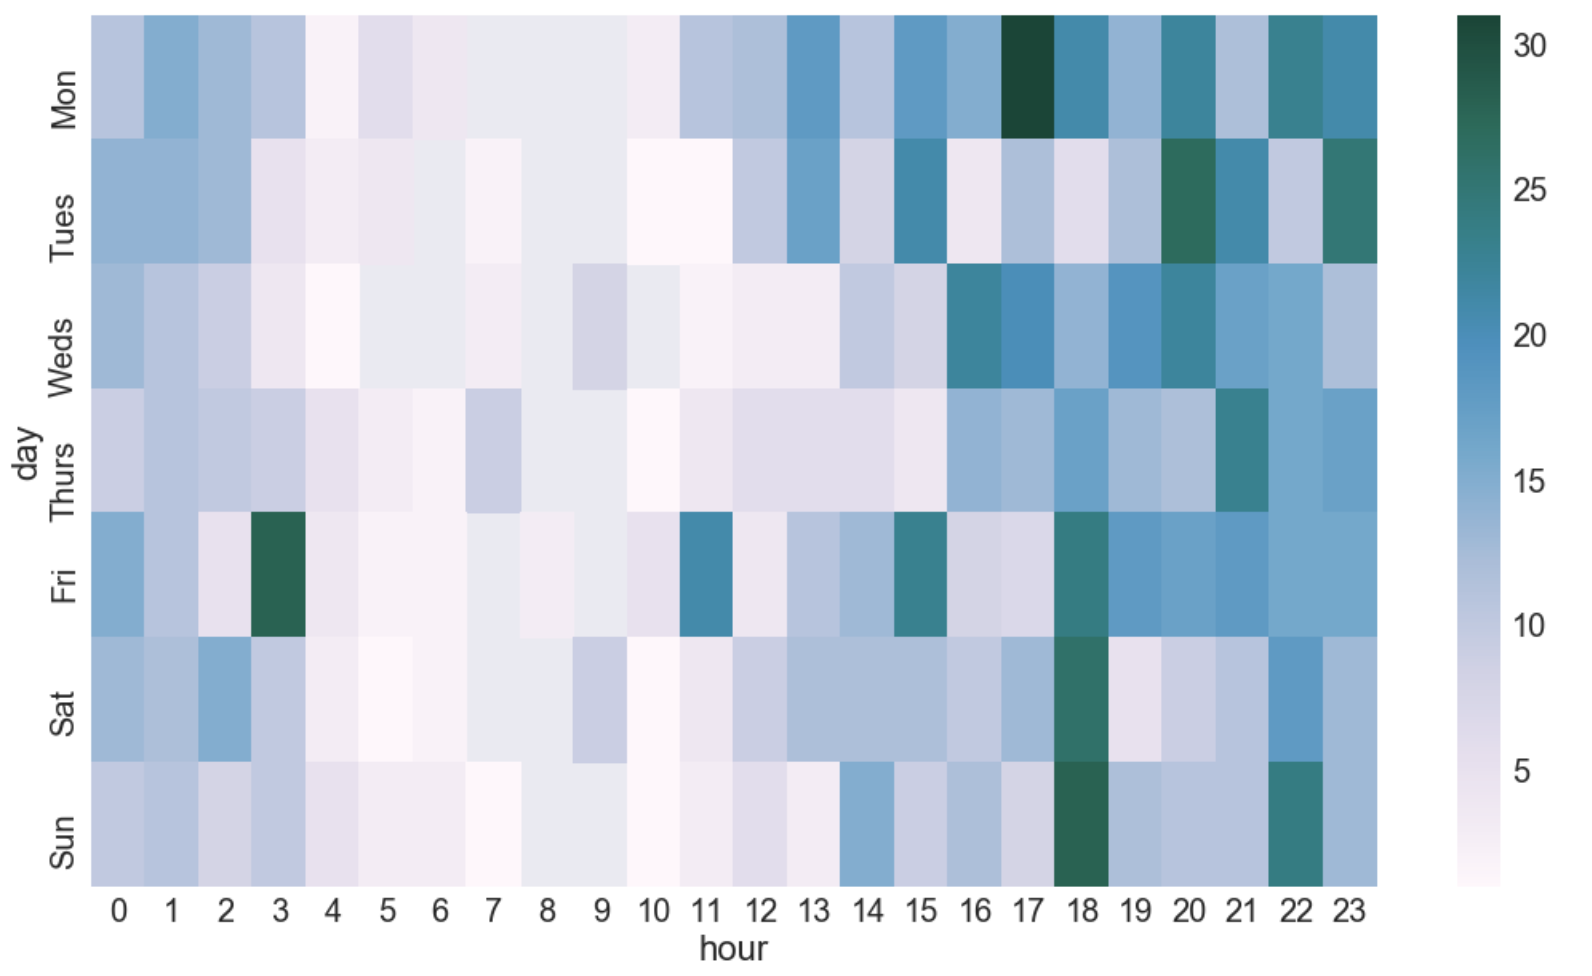
\includegraphics[width=.7\textwidth]{figures/sia_heatmap}
\caption{Number of SIA's received on day of week and hour of day.}
\label{fig:sia_heatmap}
\end{figure}

\subsection{Predictor Variables}

Mean, median, and standard deviation values for each continuous predictor variable are shown in Table~\ref{tab:descriptives}.

\begin{table}[ht]
\fontsize{11}{11.5}\selectfont \centering 
\begin{tabular}{llll}
\hline
                          & Mean & Median & Standard Deviation \\ \hline
Availability              & 3.74 & 5.00   & 1.61               \\
Importance to Participant & 3.39 & 3      & 1.38               \\
Importance to Contact     & 3.58 & 4      & 1.37               \\
Power                     & 2.68 & 2.66   & 1.07               \\
Intimacy                  & 3.43 & 3.66   & 1.33               \\ \hline
\end{tabular}
\caption{Descriptive Statistics of Continuous Predictor Variables}
\label{tab:descriptives}
\end{table}

Table~\ref{tab:correlation} shows the Pearson correlation matrix between each of the continuous predictor variables\footnote{Given high correlations between some predictor variables, examining variable inflation factor (VIF) is recommended to avoid multicollinearity in regression models. For the models specified below, VIF was calculated using the method described in \citet{zuur2009mixed} for multilevel models. All values were $< 5$, indicating multicollinearity is not problematic~\citep{sheather2009modern}.}. To better understand the relationship between the relationship between the continuous relational variables intimacy and power with the categorical proximity measure, Figures~\ref{fig:intimacy_by_distance} and \ref{fig:power_by_distance} plot the mean value for each of these continuous variables at the different proximity levels.

\begin{table}[ht] 
\fontsize{9}{9.5}\selectfont \centering 
\begin{tabular}{rlllll}
  \hline
 & Availability & Importance to Participant & Importance to Contact & Power & Intimacy \\ 
  \hline
Availability & 1 &  &  &  &  \\ 
  Importance to Participant & 0.22 & 1 &  &  &  \\ 
  Importance to Contact & 0.21 & 0.66 & 1 &  &  \\ 
  Power & 0.04 & 0.03 & -0.02 & 1 &  \\ 
  Intimacy & 0.03 & 0.06 & 0.01 & 0.65 & 1 \\ 
   \hline
\end{tabular}
  \caption{Correlation Matrix of Continuous Predictor Variables} 
  \label{tab:correlation} 
\end{table}

\begin{figure}[h]
\centering
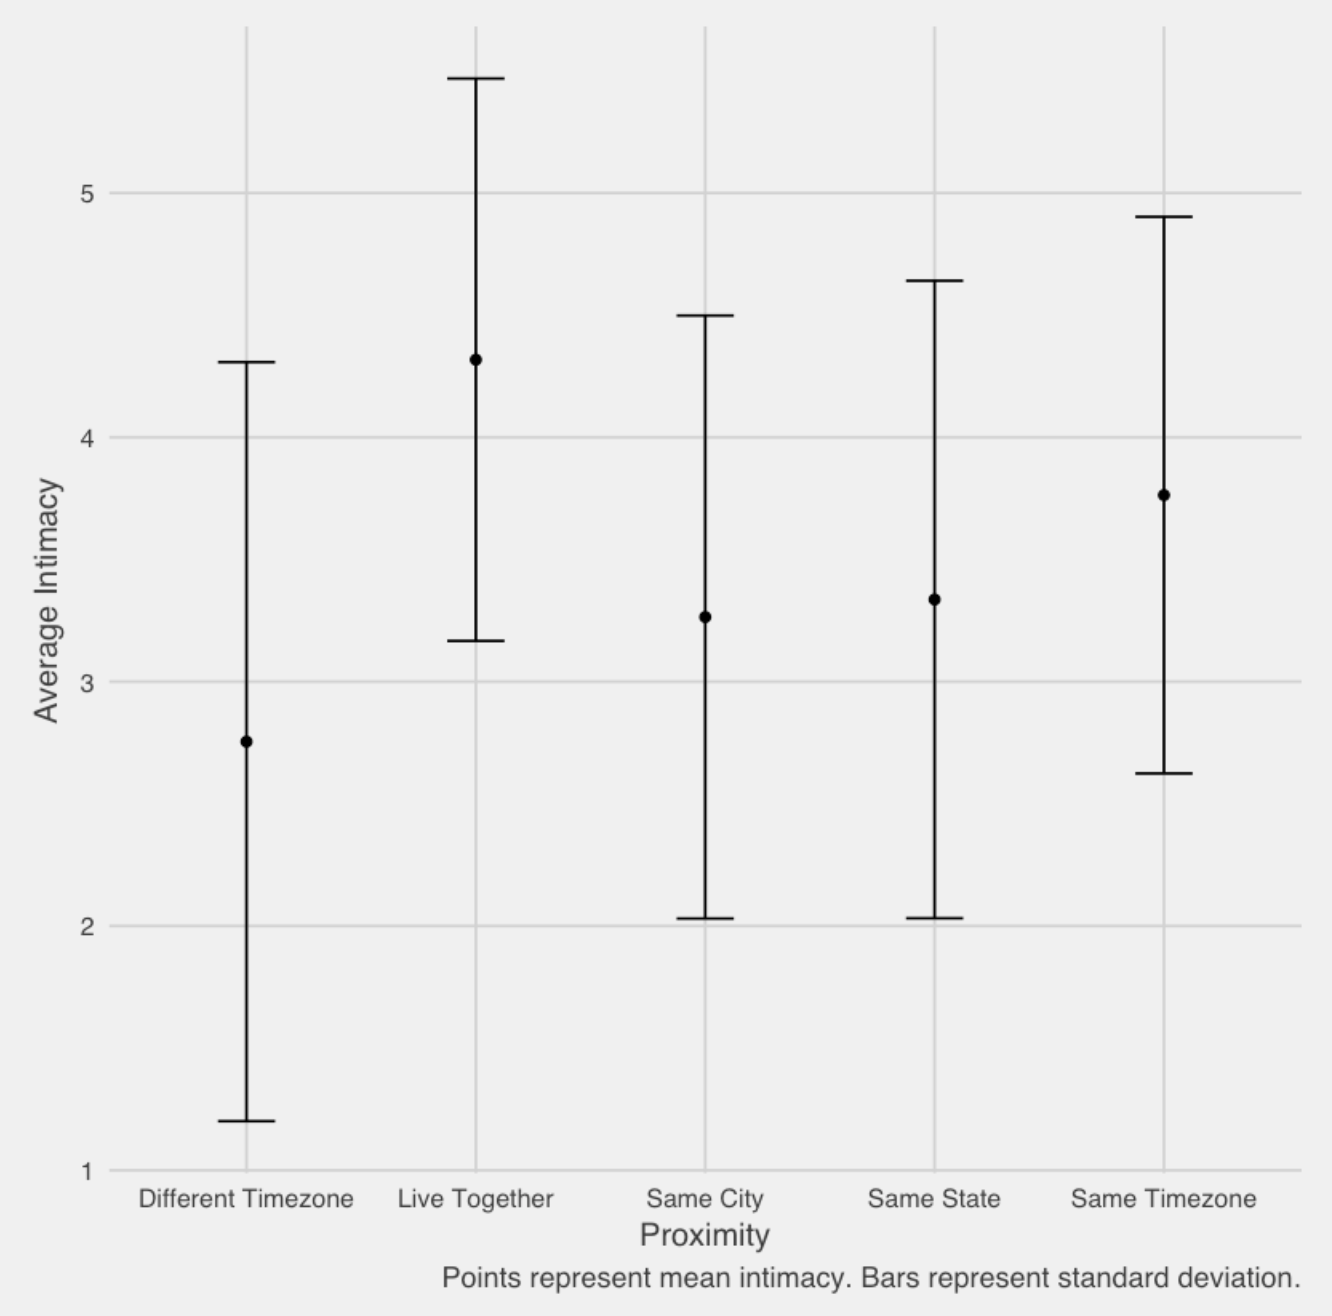
\includegraphics[width=.7\textwidth]{figures/intimacy_by_distance}
\caption{Average contact intimacy across proximity measures.}
\label{fig:intimacy_by_distance}
\end{figure}

\begin{figure}[h]
\centering
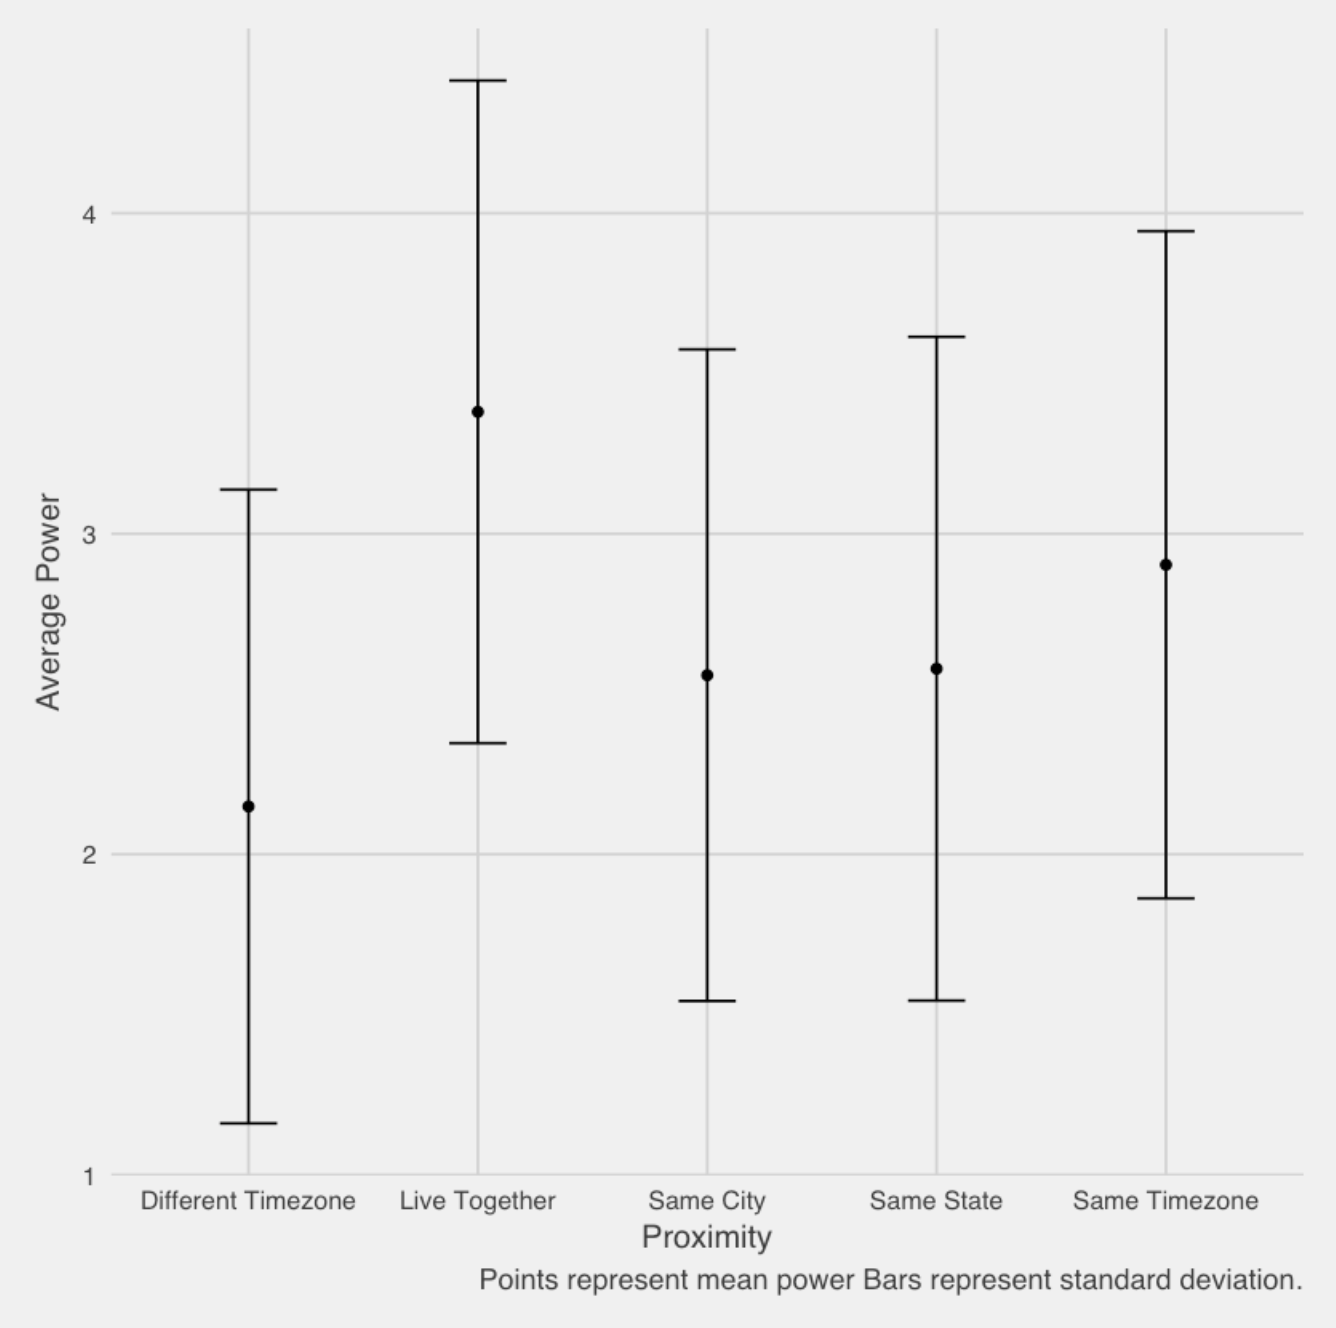
\includegraphics[width=.7\textwidth]{figures/power_by_distance}
\caption{Average power across proximity measures.}
\label{fig:power_by_distance}
\end{figure}



\section{Regression Results}

Results from the estimated regression models are shown in Table~\ref{tab:fixed_effects}. All models included age and gender as covariates. In order to control for the how active the user was in texting, the log of the number of texts a participant sent over the 1 week study period was also included as a covariate. Model 1 included these control variables as well as the 0-5 availability measure. Model 2 introduced the message content variables importance, importance to contact, and dummy variables indicating if the message was a request. Model 3 included the relational variables intimacy, power, as well as proximity. Model 4 included interactions between message content and relational variables and availability. Because the dependent variable in the regression models was the natural log of response time in seconds, the estimated $\beta$ coefficients can be interpreted as multiplicative effects on responsiveness, i.e., $(exp(\beta) - 1) \times 100 $ represents the percent change in response time.

% Table created by stargazer v.5.2 by Marek Hlavac, Harvard University. E-mail: hlavac at fas.harvard.edu
% Date and time: Thu, May 10, 2018 - 17:38:33
\begin{table}[!htbp] \fontsize{7}{7.2}\selectfont \centering 
\begin{tabular}{@{\extracolsep{5pt}}lcccc} 
\\[-1.8ex]\hline 
\hline \\[-1.8ex] 
 & \multicolumn{4}{c}{\textit{Dependent variable:}} \\ 
\cline{2-5} 
\\[-1.8ex] & \multicolumn{4}{c}{log(Response Delay in Seconds)} \\ 
\\[-1.8ex] & (1) & (2) & (3) & (4)\\ 
\hline \\[-1.8ex] 
 Age & 0.005 & 0.004 & 0.004 & 0.005 \\ 
  & (0.017) & (0.017) & (0.017) & (0.017) \\ 
  & & & & \\ 
 Gender (Male) & $-$0.210 & $-$0.286 & $-$0.329 & $-$0.326 \\ 
  & (0.287) & (0.294) & (0.295) & (0.292) \\ 
  & & & & \\ 
 log(Total Messages Sent by Participant over Study Period) & $-$0.089 & $-$0.104 & $-$0.129 & $-$0.128 \\ 
  & (0.112) & (0.114) & (0.115) & (0.114) \\ 
  & & & & \\ 
 Availability & $-$0.497$^{***}$ & $-$0.500$^{***}$ & $-$0.499$^{***}$ & $-$0.549$^{***}$ \\ 
  & (0.032) & (0.032) & (0.032) & (0.070) \\ 
  & & & & \\ 
 Importance to Participant &  & $-$0.167$^{***}$ & $-$0.173$^{***}$ & $-$0.108$^{*}$ \\ 
  &  & (0.054) & (0.054) & (0.059) \\ 
  & & & & \\ 
 Importance to Contact &  & 0.069 & 0.072 & 0.009 \\ 
  &  & (0.055) & (0.055) & (0.060) \\ 
  & & & & \\ 
 Action Request &  & 1.512$^{***}$ & 1.511$^{***}$ & 1.246$^{***}$ \\ 
  &  & (0.207) & (0.207) & (0.231) \\ 
  & & & & \\ 
 Information Request &  & $-$0.010 & $-$0.021 & $-$0.016 \\ 
  &  & (0.125) & (0.125) & (0.133) \\ 
  & & & & \\ 
 Power &  &  & 0.182 & 0.207 \\ 
  &  &  & (0.125) & (0.128) \\ 
  & & & & \\ 
 Intimacy &  &  & $-$0.049 & $-$0.061 \\ 
  &  &  & (0.099) & (0.101) \\ 
  & & & & \\ 
 Different Timezone &  &  & $-$0.041 & $-$0.082 \\ 
  &  &  & (0.331) & (0.330) \\ 
  & & & & \\ 
Live Together &  &  & $-$0.551$^{**}$ & $-$0.532 \\ 
  &  &  & (0.279) & (0.278) \\ 
  & & & & \\ 
Same State &  &  & 0.064 & 0.063 \\ 
  &  &  & (0.222) & (0.222) \\ 
  & & & & \\ 
 Same Timezone &  &  & $-$0.243 & $-$0.291 \\ 
  &  &  & (0.382) & (0.381) \\ 
  & & & & \\ 
 Availability:Importance to Participant &  &  &  & $-$0.069$^{**}$ \\ 
  &  &  &  & (0.030) \\ 
  & & & & \\ 
 Availability:Importance To Contact &  &  &  & 0.087$^{***}$ \\ 
  &  &  &  & (0.030) \\ 
  & & & & \\ 
 Availability:Action Request &  &  &  & 0.319$^{***}$ \\ 
  &  &  &  & (0.123) \\ 
  & & & & \\ 
 Availability:Information Request &  &  &  & $-$0.007 \\ 
  &  &  &  & (0.071) \\ 
  & & & & \\ 
 Availability:Power &  &  &  & $-$0.024 \\ 
  &  &  &  & (0.041) \\ 
  & & & & \\ 
 Availability:Intimacy &  &  &  & 0.007 \\ 
  &  &  &  & (0.035) \\ 
  & & & & \\ 
 Constant & 6.601$^{***}$ & 6.735$^{***}$ & 6.925$^{***}$ & 6.948$^{***}$ \\ 
  & (0.530) & (0.548) & (0.567) & (0.564) \\ 
  & & & & \\ 
\hline \\[-1.8ex] 
\\[-1.8ex] & \multicolumn{4}{c}{Random Effects Variance} \\ 
\hline \\[-1.8ex] 
 Participant & 0.760 & 0.834 & 0.809 & 0.780 \\
 Contact & 1.673 & 1.676 & 1.684 & 1.694 \\
 Residual & 2.585 & 2.462 & 2.462 & 2.443 \\
 \hline \\[-1.8ex] 
 \hline \\[-1.8ex] 
Log Likelihood & $-$3,347.506 & $-$3,320.159 & $-$3,321.296 & $-$3,325.114 \\ 
Akaike Inf. Crit. & 6,711.012 & 6,664.319 & 6,678.592 & 6,698.228 \\ 
\hline 
\hline \\[-1.8ex] 
\textit{Notes:}  & \multicolumn{4}{p{\dimexpr 0.55\linewidth-2\tabcolsep}}{ Age is centered on it's mean. All scale variables are centered at the mid-point of their scale. Female is used as the reference level for gender. Non-requests are the reference level for request type. ``Same City'' is the reference level for proximity. Parenthetical values are standard errors. $^{**}$p$<$0.05; $^{***}$p$<$0.01} \\ 
\\
\end{tabular} 
  \caption{Multilevel Regression Results} 
  \label{tab:fixed_effects} 
\end{table} 

\subsection{Robustness Checks}

Before interpreting the estimated regression models, it is useful first to ensure these effects are robust against alternative model specifications.

In examining the Model 3, intimacy has a small, nonsignificant effect, whereas the ``Live Together'' level of the proximity measure has a large, significant effect. A possible explanation for this is that participants tended to live with significant others who they rated as highly intimate, and therefore the inclusion of proximity could affect interpretation of the intimacy variable. However, removing proximity from the model only modestly increases the effect of availability (from -0.049 to -0.071) and the effect remains nonsignificant. Power is also unaffected.

Additionally, the importance to contact measure could also feasibly explain some relational effects, i.e., messages from high power contacts are more likely to be thought of as important. However, removing the importance to contact measure does not result in changes to the estimated relational effects. In Table~\ref{tab:robust_regression}.

\subsubsection{Sampling Bias}

Participants ran the data collection app on their phones for 7 days, after which no additional data was collected. One possible issue with this is under sampling messages that have long response delays due to a closing window over the sampling period. Messages that took 3 days to respond to, for example, would appear in the collected dataset if they were received within a participant's first 4 participation days, but not if they were received during the final 3.

Since only 7 days of data are collected for each participant, one way to test any potential bias is to examine a subset of the data restricted to messages received within a participant's first 3 days of running the application. Comparing this subset to the full dataset, both distributions have the same median response delay, but the 90\textsuperscript{th} percentile for the subset is 9667.87 seconds versus 7782.29 for the full dataset.

To test if this bias affects regression interpretation, Model 4 was re-fit on this subset of data. The reduction in the number of observations will result in higher standard errors, and therefore less significant effects. However, if estimated effects to this model are similar to the model above, it indicates data truncation may not result in bias in the model.

The results of re-fitting Model 4 on this subset of data are shown in the appendix in Table~\ref{tab:robust_regression}. Effects of theoretical interest remain consistent, but there are some differences in proximity effects. This appears to be because the average response delay to the ``Same city'' proximity level is larger in the restricted analysis. In other words, the data collection method results in some data truncation of long ($> 2$ days) delays, many of which are responses to to contacts who live in the same city as the participant.


\subsection{Availability}

\textit{RQ1} asked what is the relationship between a user's current availability and their mobile responsiveness. As seen in Table~\ref{tab:fixed_effects}, the availability variable has a large, significant effect on predicting mobile responsiveness.  A unit increase on the 0-5 availability scale is associated with a decrease in response time in seconds by approximately 40\% across all models.

\subsection{Message Attributes}

\textit{RQ2} asked about the relationship between message attributes and mobile responsiveness to that message. Model 2, which introduced these message attribute variables, significantly improved model fit over Model 1 which only included availability ($\chi^2(4) = 66.64$, p < .001). Participants rated messages on 1-5 scales on how important a message was to them and how important they believe the message was to the contact who sent it to them. A unit increase on the importance to participant scale is associated with a significant 15\% decrease in responsiveness. The effect of the importance to contact variable was small and insignificant.

Messages were coded as not a request, an information request, or an action request. Information requests did not differ significantly from non-requests. On the other hand, responses to action requests took approximately 4.5 times longer than responses to non-requests.


\subsection{Relational Variables}

\textit{RQ3} asked about how message sender--receiver relationship affects mobile responsiveness. Model 3 introduced the power, intimacy, and proximity variables. Power and intimacy are continuous variables measured on a 5 point scale and proximity is a factor.

These variables did not significantly improve model fit ($\chi^2(6) = 6.46$, p = .37). Responses to a contact that a participant lived with were significantly 40\% faster than to contacts who only lived in the same city as the participant, but neither power or intimacy had significant effects on responsiveness.

\subsection{Interaction Effects}

Both \textit{RQ2} and \textit{RQ3} asked how message attributes and relational variables moderate the effect of availability on mobile responsiveness. Model 4 included interaction terms between message attribute and relational variables with availability.

The inclusion of these interaction terms significantly improved model fit over the message attribute model ($\chi^2(13) = 21.00$, p = .02). Significant interactions with availability were found for both importance measures as well as action requests. Figures~\ref{fig:importance_availability_interaction},~\ref{fig:importance_contact_availability_interaction}, and \ref{fig:request_availability_interaction} plot predicted values from Model 4 to visualize these interactions.

\begin{figure}[h]
\centering
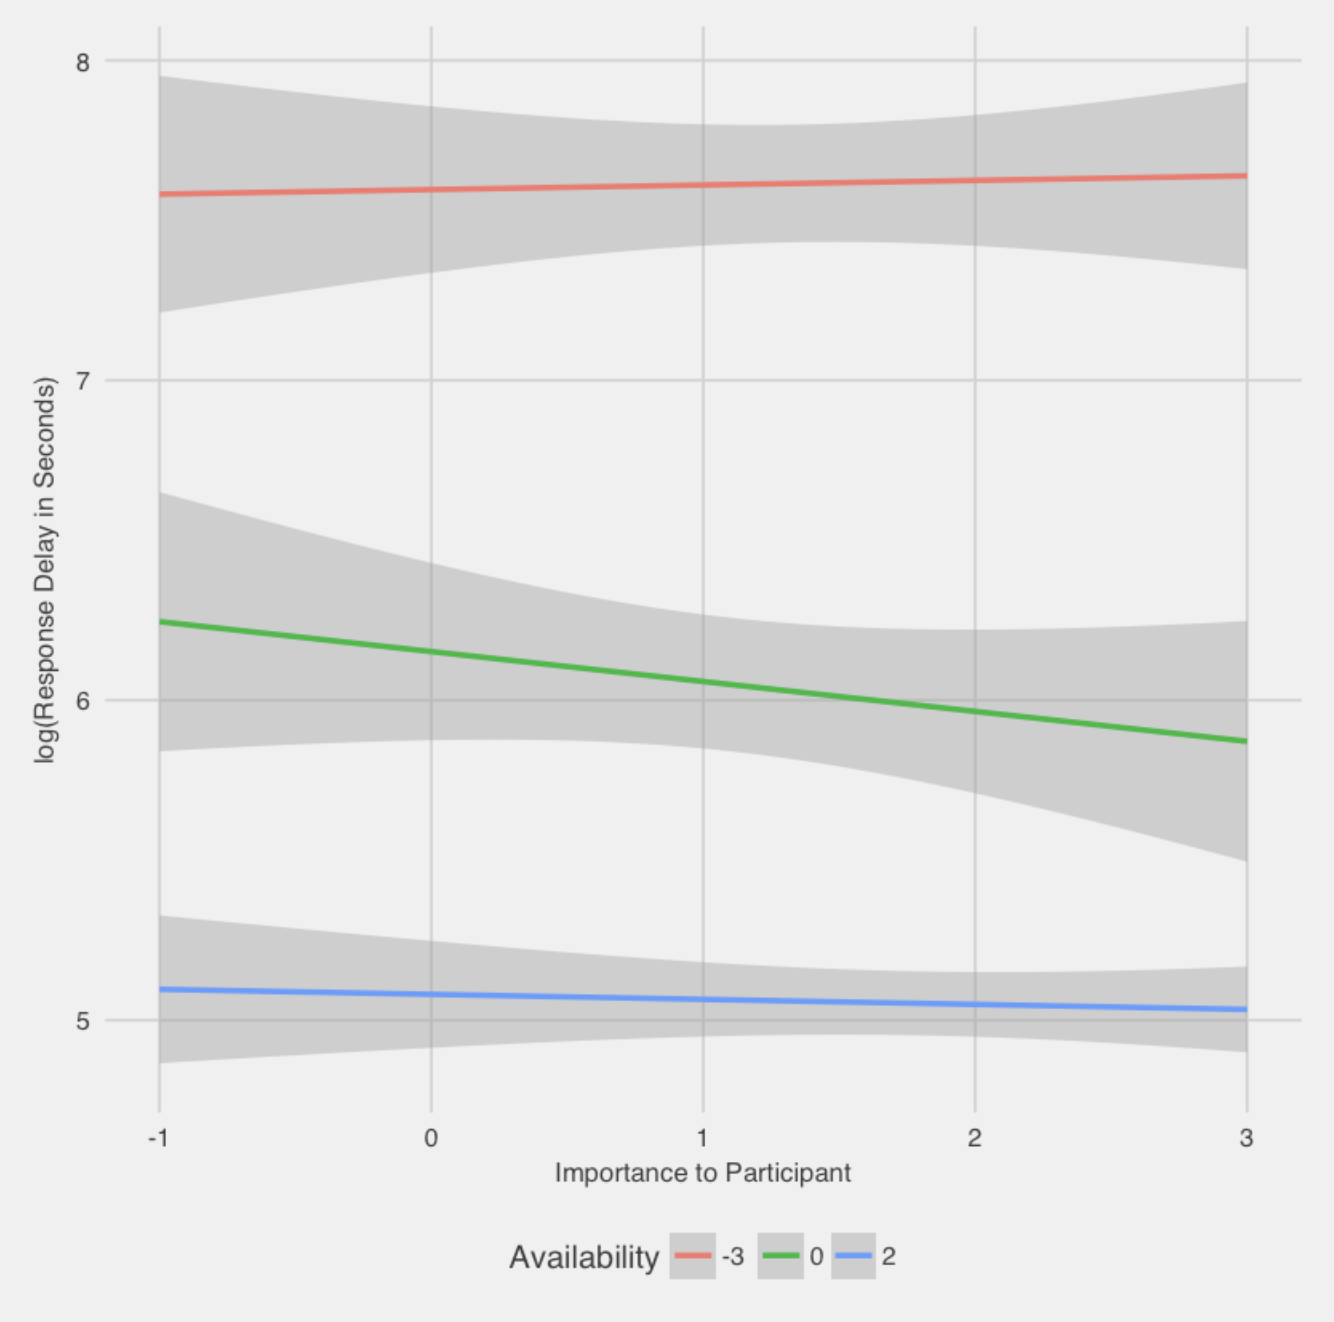
\includegraphics[width=.7\textwidth]{figures/importance_availability_interaction}
\caption{Interaction effect of availability and importance to participant on responsiveness.}
\label{fig:importance_availability_interaction}
\end{figure}

\begin{figure}[h]
\centering
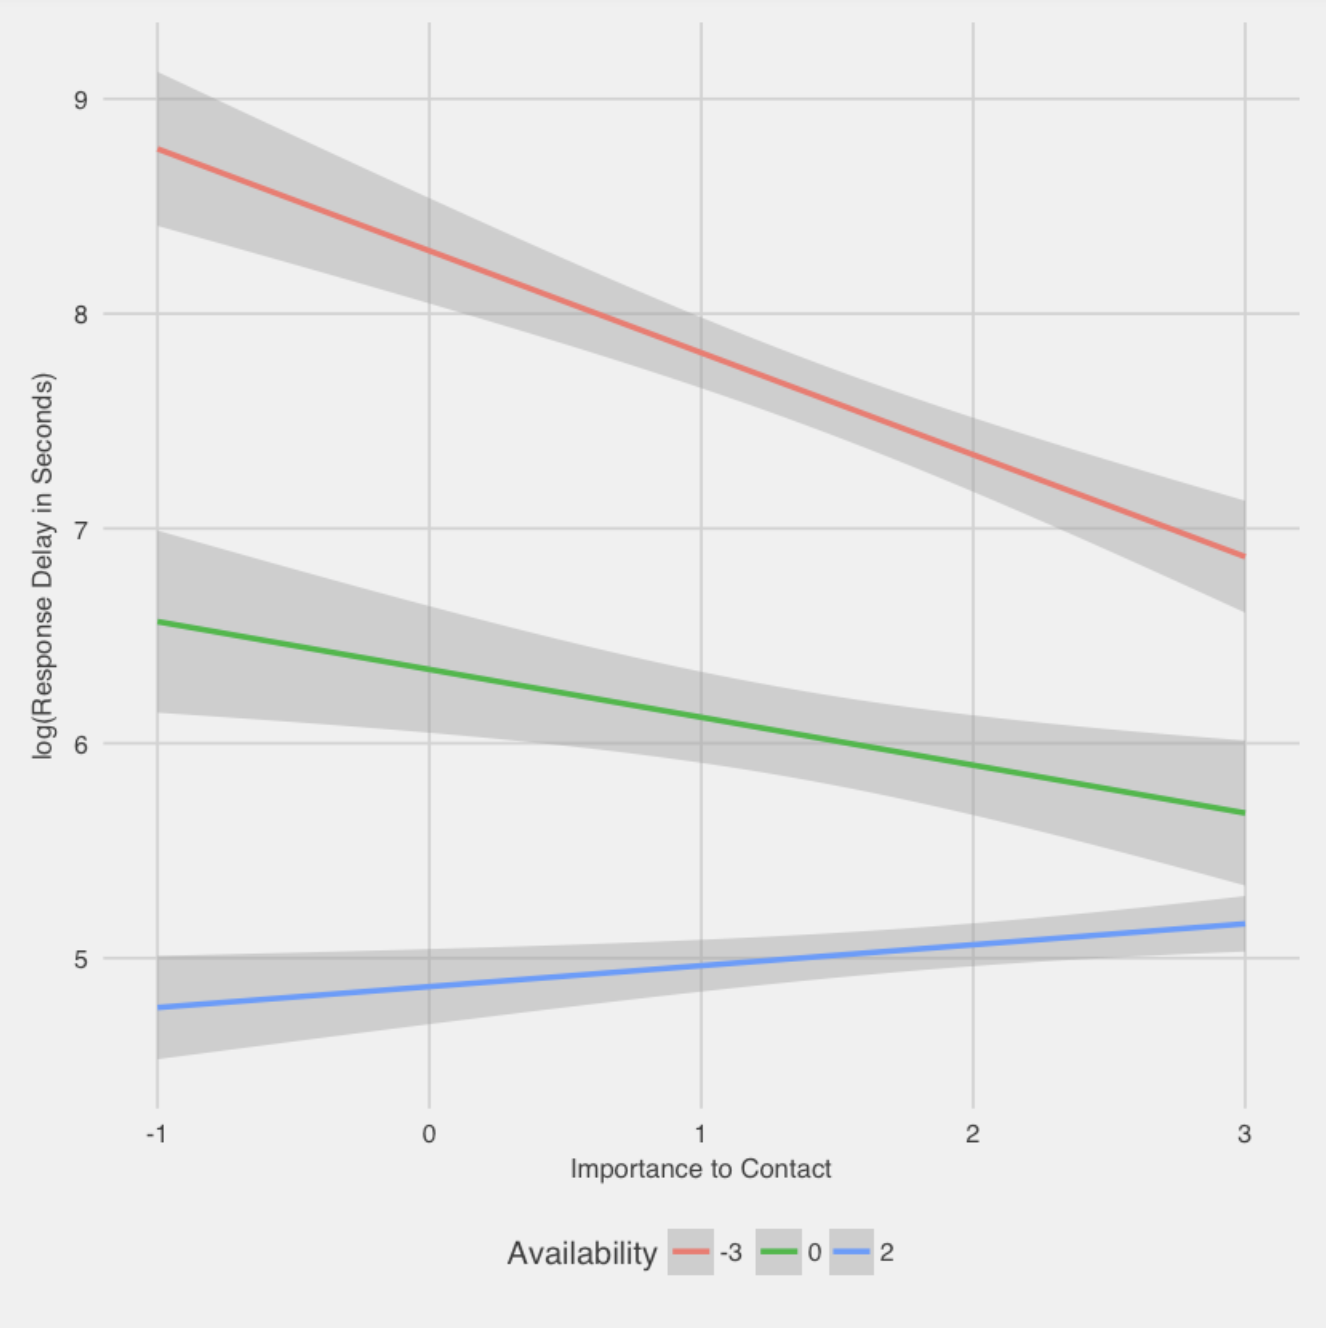
\includegraphics[width=.7\textwidth]{figures/importance_contact_availability_interaction}
\caption{Interaction effect of availability and importance to contact on responsiveness.}
\label{fig:importance_contact_availability_interaction}
\end{figure}

\begin{figure}[h]
\centering
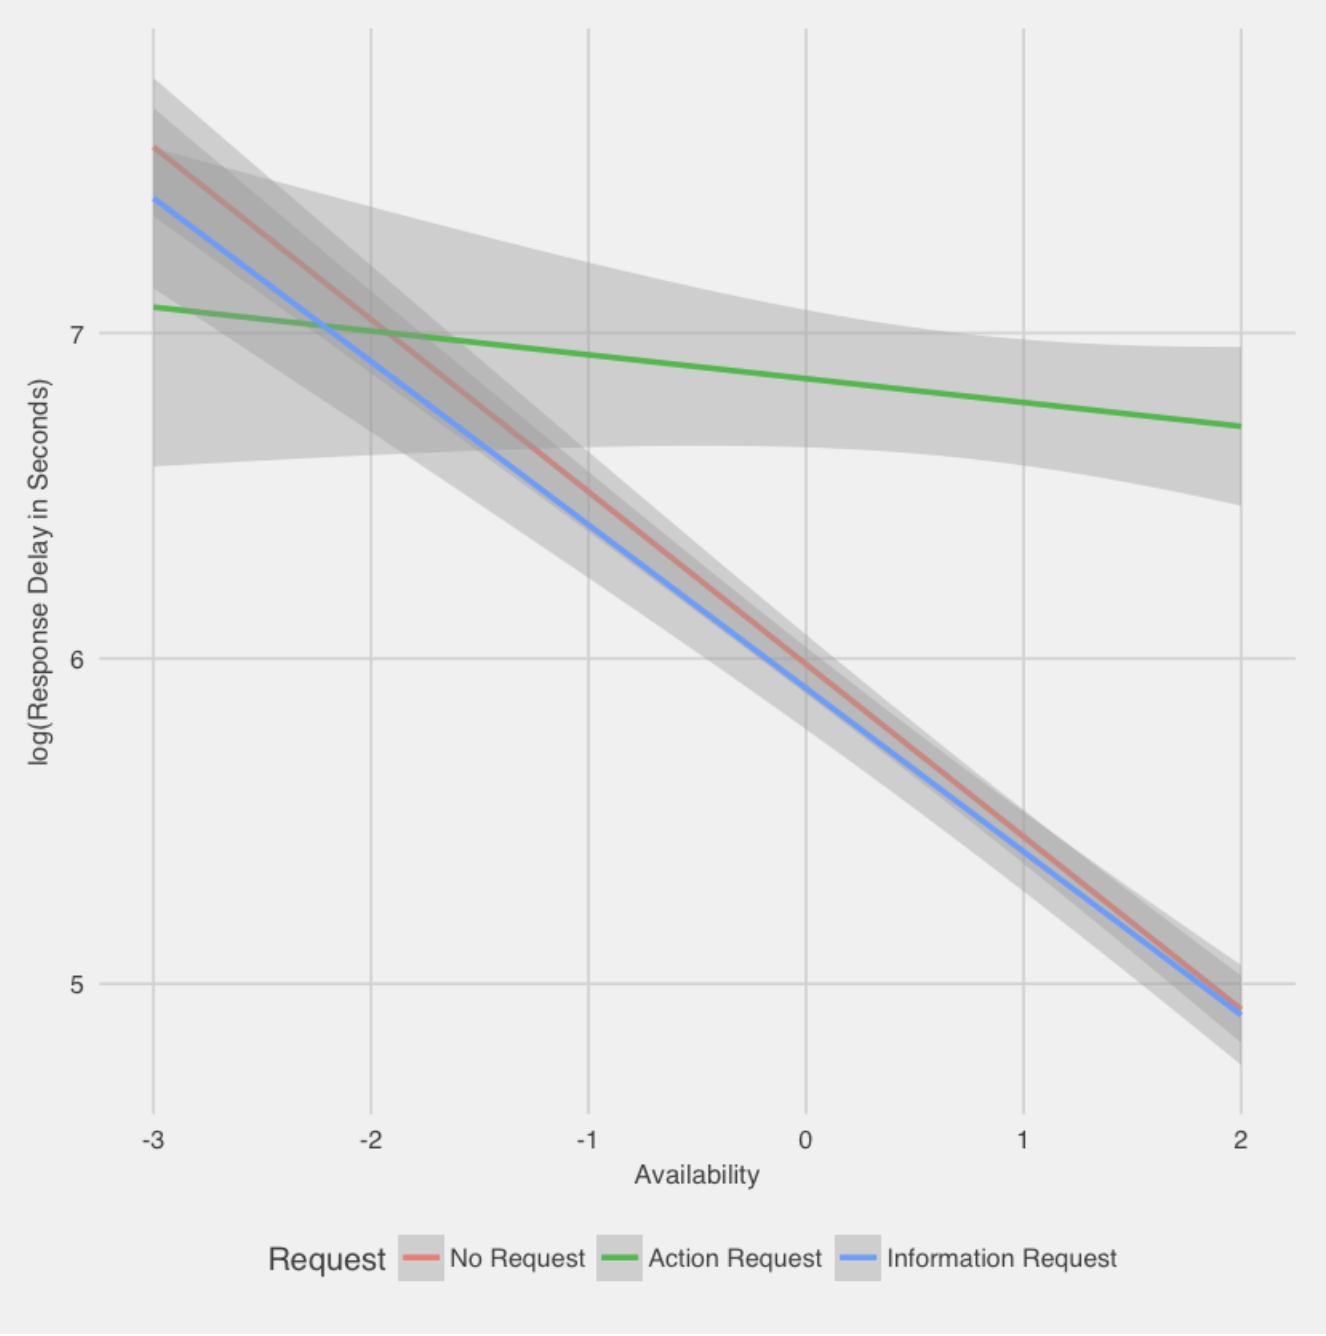
\includegraphics[width=.7\textwidth]{figures/request_availability_interaction}
\caption{Interaction effect of availability and request messages on responsiveness.}
\label{fig:request_availability_interaction}
\end{figure}


\chapter{Discussion}

The effects of the different types of variables studied -- availability, message content, and relational variables -- can be interpreted with regards to prior work on responsiveness. Taken together, these findings have both theoretical and practical implications.

\section{Availability}

Availability had a strong, consistent effect across models. Holding other variables constant, a participant who rated themselves on the lowest end of the availability scale would take an average of about 32 minutes to respond, whereas a participant who rated themselves on the highest end of the availability scale would take an average of about 2 minutes. This is one of the largest observed effects.

It is interesting also to note the interaction between availability and the importance to contact measure shown in Figure~\ref{fig:importance_contact_availability_interaction}. When participants were highly unavailable, increased importance to contact had a large effect on decreasing response time. However, when participants were highly available, importance to contact had barely any effect. This may be interpreted as that, at least for certain types of messages, participants are already very likely to respond quickly so long as they view themselves as very available, and so certain message attributes have little effect on responsiveness.

An inverse relationship between availability and response time seems fairly intuitive -- a device owner should take more time to respond if they are distracted or busy. At the same time, the strength of this effect should be considered in relation to how users have reported their own behavior in prior work. Interview participants in \citet{wohn2015ambient}, for example, described sometimes intentionally delaying response, even when they were available, to lower future expectations about responsiveness, consistent with other reports of otherwise being overwhelmed by constant connection~\citep[e.g.,][]{ames2013managing,hall2012calling}. If this were a common practice, we would expect a weaker availability effect. On the contrary, at least among participants in this study, availability was a strong predictor of responsiveness.

Outside of the regression models, also of note is just how frequently participants rated themselves on the high end of the availability scale. Participants rated themselves as a 4 or a 5 in 68\% of cases. Comparing this to the heat map figure shown in Figure~\ref{fig:sia_heatmap} may be illustrative. Figure~\ref{fig:sia_availability_heatmap} shows a similar heat map, but instead plots the mean availability for SIA's received at that time. While certain times in the morning correspond to low availability, many other times have higher values. So, in addition to availability having a large effect on responsiveness, participants also view themselves on the higher end of the availability scale fairly often.

\begin{figure}[h]
\centering
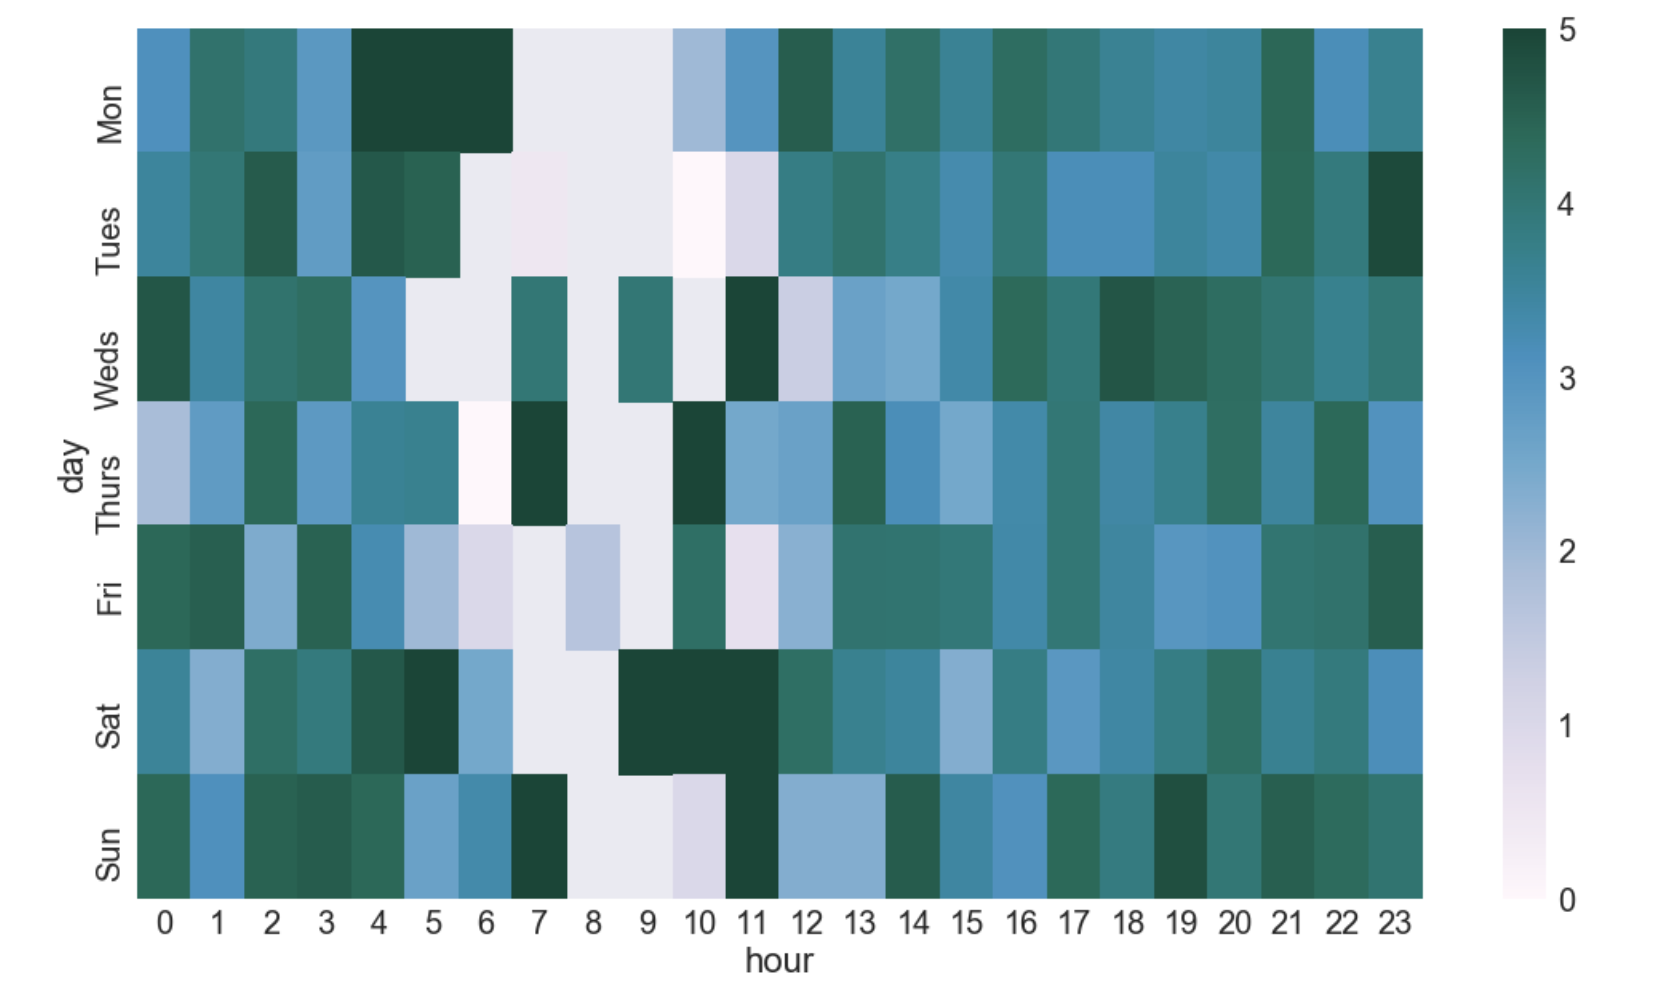
\includegraphics[width=.7\textwidth]{figures/sia_availability_heatmap}
\caption{Mean participant availability for SIA's received at day of week and hour of day.}
\label{fig:sia_availability_heatmap}
\end{figure}


\section{Message Attributes}

An increase in the importance to participant variable added in Model 2 was associated with a significant decrease in responsiveness, although this effect was much smaller than the availability effect. Holding other variables constant, a message seen as totally unimportant (a 1 on the scale) received a response on average in about 7 minutes, as opposed to a very important message, which received a response on average in just under 4 minutes.

While importance to contact did not have a significant main effect, it did have a significant interaction with availability (see Figure~\ref{fig:importance_contact_availability_interaction}). As discussed above, the effect of importance to contact becomes stronger as availability decreases. A message that was viewed as not at all important to the contact that was received when a participant was very unavailable had an average response time of about 1 hour. However, a message viewed as extremely important to the contact which was received at a time when the participant was very unavailable had an average response time of 22 minutes.

The largest message attribute effect is the type of message in the typology of requests. While non-requests received an average response of about 4.5 minutes, the average response time to action requests was around 20 minutes.  The interaction effect between request type and availability is shown in Figure~\ref{fig:request_availability_interaction}. There is no significant difference between non-requests and information requests, and we see that both of these types of messages tend to receive faster responses from more available individuals. On the other hand, even when an individual is very available, they do not generally respond to action requests as quickly.

Examples of action requests include messages like ``Wake me up at like 5.'' and ``Feed the pets later if I'm not home.'' While the data collected for this project cannot determine why responses to action requests generally take longer, one plausible explanation is that if they refer to some future action, users are able to acknowledge receipt simply by performing the action (e.g., calling the person at 5 to wake them up), rather than responding immediately.

Interview participants in \citet{wohn2015ambient} described considering certain types of messages as less urgent, and therefore not needing an immediate response. Because a text message like ``Feed the pets later if I'm not home'' refers to some future action, it may be seen as not immediately urgent. Nevertheless, many non-requests also seem not urgent, but still tended to receive faster replies when a participant was available, so urgency alone might not predict responsiveness.

Interview participants in \citet{cui2016beyond} also described message type as an important consideration in deciding when to engage with a message, However, \citet{cui2016beyond} categorizes messages as being transactional or not, viewing requests for information as distinct in being more goal-oriented, and associated with faster responses. This is in contrast to my findings, where only action requests differed from non-requests, and resulted in longer response times.

My findings support these qualitative findings that responsiveness is adjusted based on different types of messages. However, message attributes such as urgency and distinctions such as ``goal-oriented'' or ``task-based'' may not be the best way to think about how message type affects responsiveness. What distinguishes action requests in this data set is that they ask a participant to do some non-texting action. \citet{rettie2009mobile} discusses SMS, phone calls, and email in terms of the boundaries of asynchronous and synchronous interaction, arguing that norms govern the perceived synchronicity of a medium (e.g., email is seen as a largely asynchronous medium whereas instant messaging is seen as a synchronous medium -- not for technical reasons so much as social norms governing their use). This may provide a useful theoretical starting point to interpret these findings. It may be that when an SMS interaction ``stays'' within the boundaries of texting, it is seen as facilitating nearly synchronous exchanges, but when a conversation requests non-texting action, the conversation norms then move outside the norms of texting.

\section{Relational Variables}

Relational variables largely did not have an effect on responsiveness. The effects of power and intimacy were non-significant. In Model 3, responses to a contact that the participant lived with differed significantly from responses to a contact that lived in the same city, with response time decreasing an average of about 40\%. This effect was slightly smaller and not significant in the more complex Model 4.

The estimated variance parameters for our random effects of participant and contact are of note here. In Model 4, between-participant variance was estimated as $0.780$, whereas within-participant between-contact variance was estimated as $1.694$. In other words, participants varied more in responsiveness in how they responded to different contacts than than did when compared to one another, which would suggest there are between-contact differences that are just not accounted for by the relational variables collected.

It should be noted, however, that participants' SIA distribution is similar to the skewed message distribution shown in Figure~\ref{fig:received_messages_by_contact}. In other words, if an average participant received 12 SIA's over the study period from 4 contacts, typically 8-9 of those would be received from one contact while the rest of the contacts would only have sent 1 or 2. As a result, most contacts in the collected data contain few SIA observations.

Power and intimacy were chosen as they are commonly associated with models of relational work in communication~\citep{brown1987politeness,spencer2011conceptualising}, and if responsiveness is guided in part by normative expectations, it seemed possible that these relational considerations that often affect normative behavior in FtF interaction~\citep[e.g.,][]{guerrero1991waxing,henley1973power,leffler1982effects,sternglanz2004reading} would also affect this CMC behavior.

However, CMC, and mobile messaging in particular, offers communicators certain affordances not present in FtF conversation. One of these is \textit{plausible deniability}~\citep{lederer2004personal,nardi2000interaction}. This allows a device owner to, for example, temporarily ignore a message and then later use a white lie to explain their behavior (e.g., ``Sorry, I just saw your  message!'')~\citep{hancock2009butler}. Although participants tended to respond more quickly when they were available, they may not feel governed in mobile messaging by the same types of factors that affect normative behavior otherwise.

\section{Theoretical Implications}

\subsection{Social Information Processing}

Social Information Processing~\citep{walther1992interpersonal} suggests CMC users adapt to their communication medium and find ways to encode social and relational information in the style and timing of the messages they send. \citet{walther1995nonverbal} and \citet{kalman2006pauses} hypothesized responsiveness was one cue communicators use to convey intimacy and presence in CMC.

On one hand, the failure to find a large relational effect in the regression models could indicate this is not the case -- at least not for SIA messages. If responsiveness was used to indicate closeness, we would expect on average that contacts who were rated higher in intimacy to receive quicker responses.

On the other hand, the modest effects of the message importance measures could be related to a SIP process. We know that CMC communicators interpret certain lexical cues as relating to heightened urgency~\citep{nguyen2014lexical,nguyen2016effects} or desiring faster responses~\citep{cui2016beyond}. As seen in Figure~\ref{fig:importance_contact_availability_interaction}, when participants are unavailable, higher levels of importance to contact are associated with quicker responses. From a SIP perspective, it could be that mobile messaging users recognize cues indicating a message is important to the person contacting them, and update their responsiveness appropriately.

Still, this effect is strongest when users are largely unavailable. So while faster responses could mean a user is reacting to a cue in a received message, it could also just mean the user happened to be available to respond. As such, while responsiveness may sometimes be considered a cue (e.g., ``I am busy, but I am responding as soon as I can because I know this is important to you.''), it often just signals availability.

\subsubsection{Impressions of Others}

This is especially interesting to consider in terms of work describing how responsiveness is interpreted. Mobile messaging users have described delays in response as meaningful~\citep{rettie2009mobile}, and often desire quick responses~\citep{church2013s}. Failure to meet responsiveness expectations has been shown to cause negative impressions in email~\citep{kalman2013online} and instant messaging~\citep{heston2017worth}.

In SIP terms, we can think of responsiveness as being ``decoded'' as meaningful, where delays in response are assumed to be deliberate and carry social meaning. My results suggest it is more likely a message recipient was simply not available to respond. Even messages seen as very important to a message sender still took an average of 22 minutes to respond to by highly unavailable participants -- far longer than the desired immediate response described by interview participants in the above study.

As such, responsiveness may represent one avenue to think about misunderstandings in CMC, or to use SIP language, to understand cues where the decoding and encoding processes are largely different. \citet{cramton2002attribution} discussed misunderstandings about responsiveness among virtual team members as attribution error. In other words, while workers were likely to cite external factors when describing their own ability to respond quickly to a message, when others did not respond quickly to them, they often made value judgements about their co-workers based on their response delays. This may also describe mismatches between responsiveness behavior in mobile messaging as well.

\subsection{Perpetual Contact}

A motivating argument for this work was that while responsiveness has long been considered important in CMC~\citep[e.g.][]{avrahami2006responsiveness,dabbish2005understanding,kalman2006pauses,kalman2013online,tyler2003can,walther1995nonverbal}, mobile responsiveness represents a fundamentally different problem, because mobile users can be contacted anywhere at any time, and often use their device to communicate with many different types of contacts. In other words, the decision of when to respond now occurs in a world of perpetual contact~\citep{katz2002perpetual}.

\citet{bayer2015connection} argue that constant connection has become a societal norm, and as such, we have developed habits which lead us to constantly checking our devices. My data cannot speak directly to to such claims. It is interesting to note, however, that participants marked themselves as the highest level of availability 50\% of the time, and as shown in Figure~\ref{fig:sia_availability_heatmap}, average availability was relatively high throughout many times of the day. So while my data cannot directly support sociological arguments about connection norms or mobile habits, we do see evidence that device owners' subjective assessments of availability throughout the day tends to be high, which may be of interest to future work investigating attention and mobile devices.

It is also worth noting that users have reported turning off their phones or using airplane mode to get a break from constant connection~\citep{ames2013managing,smith2015us}. Availability was shown to have a strong effect on predicting responsiveness. While participants often rated themselves high on the availability scale, it is possible that some instances of low availability represent users deliberately leaving their phones unattended, although because users were not asked to specify why they chose the availability level they did, this is not necessarily true.

However, the data does provide some evidence for prior work. In qualitative studies, mobile owners have discussed prioritizing messages based on message content to deal with the ``always on'' nature of mobile messaging~\citep[e.g.,][]{cui2016beyond,wohn2015ambient}. My results support previous findings on message content -- in my data, action requests seem to be determined low priority as far as needing immediate response. So although availability had a large effect on responsiveness, users did not simply always respond to every type of message if they were available. As such, there does seem to be some sort of prioritization happening, although not necessarily considering sender--receiver relationship, which has been noted elsewhere~\citep{laursen2005please,wohn2015ambient}.

Taken together, my findings do suggest that users are in many ways ``always on,'' but availability is not the sole factor in determining responsiveness. There are times where users rate themselves as available to respond to a message, but still choose to wait.


\section{Practical Implications}

My findings also have practical implications for the design of mobile messaging platforms. Research in CSCW and HCI has attempted to build predictive models of responsiveness~\citep[e.g.,][]{avrahami2007improving,avrahami2008waiting,dabbish2005understanding}, in part to build better awareness displays. Especially within the workplace, it has been demonstrated that displaying a potential message recipient's current work status to a message sender can allow the sender to better time their message and not interrupt the recipient at an inopportune time (i.e., if the recipient is in the middle of a very focused task, the sender may delay sending the message as to not interrupt and disrupt the recipient)~\citep{dabbish2004awareness}. Predictive systems that can infer how busy a worker is would be useful in automatically setting an awareness display.

Recently, \citet{pielot2014didn} suggested a similar system for mobile messaging applications. They suggest displaying to a message sender the likelihood of receiving a quick response, motivated less by reducing interruptions and distractions, and instead mitigating the negative effects of the recipient violating responsiveness expectations by giving the message sender a more realistic expectation of when to expect a response. This is done through machine learning, using phone activity as features in the machine learning model to predict the likelihood of a user seeing a message and therefore responding to it quickly.

In some ways, my results validate this approach. Responsiveness was strongly correlated with availability in my results, and the features used by \citet{pielot2014didn} (such as time of day, when the screen was last on, etc.) should be good indicators of availability. Had relational variables had a stronger effect, there might be higher concern that such a model lacked an understanding of relationship effects.

Nevertheless, the distribution of messages across contacts and the relatively high contact-level variance may be useful to consider. Within my sample, participants tended to have one or two contacts they texted with a lot, and many contacts that they texted with a lot more rarely. It may be that a machine learning model is very good at learning responsiveness behavior for an individual's top few most texted with contacts, but that these predictions are not as useful for contacts that text much more rarely. If the goal of such a system is to mitigate negative effects stemming from responsiveness expectations, it should perhaps be much more conservative in its estimates displayed to these less communicated with contacts.

Finally, action requests received significantly slower responses than other types of messages. As such, predictive models such as that in \citet{pielot2014didn} may also want to consider lexical features of a received message, which could increase model performance.

\section{Limitations and Future Work}

To the best of my knowledge, this study is the first to use a custom developed application to collect both ESM data and SMS log data to study mobile responsiveness with naturalistic data. While the findings contribute to our understanding of mobile responsiveness, they should be considered in light of the following limitations, which present opportunities for future work. 

The first is that this study focused only on SIA's, and importantly, only SIA's that received a response during the study period. The decision to focus on SIA's was that they represent a unique moment in deciding whether or not to engage with a message, as once a mobile messaging user is already involved in a conversation, they tend to respond quickly. Nevertheless, SIA messages made up only about 15\% of total messages collected. Once a user is engaged in conversation, expectations about responsiveness likely change, and different considerations may be made when considering when to respond. For example, models of SIA responsiveness reported here largely found no relational effects. It may be, however, that after a user engages with an SIA, response time to more intimate friends is faster than with less intimate acquaintances. Qualitative work that has participants review previous conversations~\citep[e.g.,][]{cui2016beyond} is useful for understanding responsiveness for these messages. Future work could potentially have participants retroactively rate many messages in a conversation on various scales for quantitative analysis. The experience sampling approach taken in the current study is likely unsuitable for studying conversations as they occur, as participants would not want to continually answer questions about every text they receive during a conversation.

Participants were asked to answer questions about an SIA at the moment of responding to it. This was done, in part, as it ensured that participants were already on their device having just responded to a message, and therefore were available to fill out a questionnaire. In addition, the goal was to not influence participant behavior toward text messages. Had the questionnaire been sent at the moment an SIA was received, a user would receive 2 different notifications about a single message, which could possibly draw more attention to a message and change their response behavior (i.e., by encouraging them to respond more quickly after receiving back to back notifications about it). However, as a result, any SIA which did not receive a response in turn never delivered the ESM questionnaire. The results presented then should be interpreted in terms of factors which effect responsiveness for messages which eventually get a response. This leaves open the question of why a mobile messaging user might never respond to a message, or at least not respond for over 1 week. A study similar to the one presented here could be used and ask participants to retroactively fill out questionnaires for SIA's never responded to during the study period at the end of the study period. However, this does run a risk of participants having recall issues discussing texts that they received over a week ago. Future studies relying only on log data, however, could be useful and avoid recall issues.

Participants for this study were somewhat diverse. Males and females were both represented, and participants of different ages were represented in the sample. Participants also represented a range of texting use, with the average participant texting a modest amount over the study period with some very heavy users. However, participants were requested from urban areas using online ads, which certainly precludes many different populations. To get a more complete understanding of mobile responsiveness, future work could focus on recruiting from more specific populations, such as rural users or older adults.

Some unexpected findings from this study suggest useful avenues for future research. When responding to an SIA, participants rated their availability at the time they received the message on a 0--5 scale. Participants rated themselves as either a 4 or 5 on this scale 68\% of the time. In this study, no other data around availability was collected to better understand why users think of themselves as available so often. Future work could collect similar scale data, but also ask users more about their current context to get a better sense of what availability actually means to users when making responsiveness decisions.

The lack of difference in responsiveness between non-requests and information requests compared to the large difference between non-requests and action requests is noteworthy. As discussed above, this suggests that some suggests typologies of mobile messages may not fully explain how users think about message content and how it affects their responsiveness behavior. Qualitative work is useful for better understanding why this is the case.

Finally, it should be noted that modeling observed naturalistic behavior is useful for understanding mobile responsiveness as it occurs in the world, but there are many questions this approach cannot answer. As indicated by the large variance terms in the above models, mobile responsiveness is complex and cannot be perfectly explained with the variables discussed here. While it is certainly useful to measure the average effects of different types of variables, these models necessarily lack the nuance gained from qualitative studies. Throughout this discussion, I have noted various areas where the observed effects in regression models differed from what would be expected based on qualitative findings. These differences may be useful in preparing future qualitative work. Furthermore, observational studies also necessarily include very noisy data. Controlled experiments would be a useful next step in better understanding how variables explored here cause differences in responsiveness. While lab-based experiments will likely have a difficult time truly capturing the mobile context, they may nevertheless be useful in measuring some of these effects in a controlled setting~\citep[see e.g.,][]{avrahami2007improving}. Novel quasi-experimental designs could also be useful~\citep[e.g.,][] {tsapeli2015investigating}.

\chapter{Conclusion}

This study was conducted to understand the effects of availability, message attributes, and relational variables on mobile responsiveness. Results indicated that in many cases, availability is strongly associated with responsiveness, but this is not true for all types of messages. These results should be of interest to CMC scholars, where results did not strongly support hypotheses of responsiveness as a nonverbal cue in CMC, and responsiveness studies could provide an entry point to thinking more about misunderstandings in how cues are constructed by a sender and interpreted by a receiver. These results should also be of interest broadly to scholars of mobile device use, as they provide some evidence of how users may choose to prioritize certain messages in a world of perpetual contact. Finally, HCI scholars interested in the design of mobile messaging platforms, and especially predictive systems to display information about message recipients, will find useful information in these results related to when their systems might fail and what other types of features may be useful to consider when predicting responsiveness.

 \renewcommand\refname{\begin{centering}References\end{centering}}
 \bibliography{references.bib}
 \bibliographystyle{apacite} %or another suitable style.



%\appendices		% Appendix begins here (optional).

\begin{appendix}
	
\chapter{Regression Model on Subset of Data}

\begin{table} \fontsize{5.5}{5.8}\selectfont \centering 
\begin{tabular}{@{\extracolsep{5pt}}lc} 
\\[-1.8ex]\hline 
\hline \\[-1.8ex] 
 & \multicolumn{1}{c}{\textit{Dependent variable:}} \\ 
\cline{2-2} 
\\[-1.8ex] & log(Response Delay in Seconds) \\ 
\hline \\[-1.8ex] 
 Age & 0.008 \\ 
  & (0.021) \\ 
  & \\ 
 Gender (Male) & $-$0.327 \\ 
  & (0.334) \\ 
  & \\ 
 log(Total Messages Send by Participant over Study Period) & $-$0.100 \\ 
  & (0.129) \\ 
  & \\ 
 Availability & $-$0.430$^{***}$ \\ 
  & (0.098) \\ 
  & \\ 
 Importance to Participant & $-$0.175$^{**}$ \\ 
  & (0.083) \\ 
  & \\ 
 Importance to Contact & 0.124 \\ 
  & (0.082) \\ 
  & \\ 
 Action Request & 0.752$^{**}$ \\ 
  & (0.316) \\ 
  & \\ 
 Information Request & $-$0.167 \\ 
  & (0.209) \\ 
  & \\ 
 Power & 0.172 \\ 
  & (0.183) \\ 
  & \\ 
 Intimacy & $-$0.030 \\ 
  & (0.143) \\ 
  & \\ 
 rDifferent Timezone & 0.232 \\ 
  & (0.473) \\ 
  & \\ 
Live Together & $-$0.683$^{*}$ \\ 
  & (0.364) \\ 
  & \\ 
Same State & 0.038 \\ 
  & (0.320) \\ 
  & \\ 
Same Timezone & $-$1.083$^{**}$ \\ 
  & (0.533) \\ 
  & \\ 
 Availability:Importance to Participant & $-$0.125$^{***}$ \\ 
  & (0.043) \\ 
  & \\ 
 Availability:Importance to Contact & 0.040 \\ 
  & (0.041) \\ 
  & \\ 
 Availability:Action Request & 0.445$^{***}$ \\ 
  & (0.170) \\ 
  & \\ 
 Availability:Information Request & 0.076 \\ 
  & (0.108) \\ 
  & \\ 
 Availability:Power & $-$0.053 \\ 
  & (0.070) \\ 
  & \\ 
 Availability:Intimacy & $-$0.015 \\ 
  & (0.054) \\ 
  & \\ 
 Constant & 7.005$^{***}$ \\ 
  & (0.659) \\ 
  & \\ 
\hline \\[-1.8ex] 
Observations & 786 \\ 
Log Likelihood & $-$1,624.176 \\ 
Akaike Inf. Crit. & 3,296.353 \\ 
Bayesian Inf. Crit. & 3,408.360 \\ 
\hline 
\hline \\[-1.8ex] 
\textit{Note:}  & \multicolumn{1}{r}{$^{**}$p$<$0.05; $^{***}$p$<$0.01} \\ 
\end{tabular} 
  \caption{Multilevel Regression Results Fit on Subset of Data} 
  \label{tab:robust_regression} 
\end{table} 

\end{appendix}


%\appendices	        % If more than one appendix chapters,
				% use appendices instead of appendix




\end{document}

